% Copyright 2010 by Till Tantau
% Copyright 2011 by Jannis Pohlmann
%
% This file may be distributed and/or modified
%
% 1. under the LaTeX Project Public License and/or
% 2. under the GNU Free Documentation License.
%
% See the file doc/generic/pgf/licenses/LICENSE for more details.


\section{Specifying Graphs}
\label{section-library-graphs}

\subsection{Overview}

\tikzname\ offers a powerful path command for specifying how the nodes in a
graph are connected by edges and arcs: The |graph| path command, which becomes
available when you load the |graphs| library.

\begin{tikzlibrary}{graphs}
    The package must be loaded to use the |graph| path command.
\end{tikzlibrary}
%
\begin{codeexample}[setup code,hidden]
    \usetikzlibrary{graphs}
\end{codeexample}

In this section, by \emph{graph} we refer to a set of nodes together with some
edges (sometimes also called arcs, in case they are directed) such as the
following:
%
\begin{codeexample}[]
\tikz \graph { a -> {b, c} -> d };
\end{codeexample}

\begin{codeexample}[preamble={\usetikzlibrary{graphs.standard}}]
\tikz \graph {
  subgraph I_nm [V={a, b, c}, W={1,...,4}];

  a -> { 1, 2, 3 };
  b -> { 1, 4 };
  c -> { 2 [>green!75!black], 3, 4 [>red]}
};
\end{codeexample}

\begin{codeexample}[]
\tikz
  \graph [nodes={draw, circle}, clockwise, radius=.5cm, empty nodes, n=5] {
    subgraph I_n [name=inner] --[complete bipartite]
    subgraph I_n [name=outer]
  };
\end{codeexample}

\begin{codeexample}[]
\tikz
  \graph [nodes={draw, circle}, clockwise, radius=.75cm, empty nodes, n=8] {
    subgraph C_n [name=inner] <->[shorten <=1pt, shorten >=1pt]
    subgraph C_n [name=outer]
  };
\end{codeexample}

\begin{codeexample}[width=6.6cm]
\tikz [>={To[sep]}, rotate=90, xscale=-1,
       mark/.style={fill=black!50}, mark/.default=]
  \graph [trie, simple,
          nodes={circle,draw},
          edges={nodes={
              inner sep=1pt, anchor=mid,
              fill=graphicbackground}}, % yellowish background
          put node text on incoming edges]
    {
      root[mark] -> {
        a -> n -> {
          g [mark],
          f -> a -> n -> g [mark]
        },
        f -> a -> n -> g [mark],
        g[mark],
        n -> {
          g[mark],
          f -> a -> n -> g[mark]
        }
      },
      { [edges=red] % highlight one path
        root -> f -> a -> n
      }
    };
\end{codeexample}

The nodes of a graph are normal \tikzname\ nodes, the edges are normal lines
drawn between nodes. There is nothing in the |graphs| library that you cannot
do using the normal |\node| and the |edge| commands. Rather, its purpose is to
offer a concise and powerful way of \emph{specifying} which nodes are present
and how they are connected. The |graphs| library only offers simple methods for
specifying \emph{where} the nodes should be shown, its main strength is in
specifying which nodes and edges are present in principle. The problem of
finding ``good positions on the canvas'' for the nodes of a graph is left to
\emph{graph drawing algorithms}, which are covered in Part~\ref{part-gd} of
this manual and which are not part of the |graphs| library; indeed, these
algorithms can be used also with graphs specified using |node| and |edge|
commands.
%
\ifluatex
As an example, consider the above drawing of a trie, which is drawn without
using the graph drawing libraries. Its layout can be somewhat improved by
loading the |layered| graph drawing library, saying |\tikz[layered layout,...|,
and then using Lua\TeX, resulting in the following drawing of the same graph:
\medskip

\tikz [layered layout, >={To[sep]}, rotate=90, xscale=-1,
       mark/.style={fill=black!50}, mark/.default=]
  \graph [trie, simple, sibling distance=8mm,
          nodes={circle,draw},
          edges={nodes={
              inner sep=1pt, anchor=mid, fill=white}},
          put node text on incoming edges]
    {
      root[mark] -> {
        a -> n -> {
          g [mark],
          f -> a -> n -> g [mark]
        },
        f -> a -> n -> g [mark],
        g[mark],
        n -> {
          g[mark],
          f -> a -> n -> g[mark]
        }
      },
      { [edges=red] % highlight one path
        root -> f -> a -> n
      }
    };
\medskip
\fi

The |graphs| library uses a syntax that is quite different from the normal
\tikzname\ syntax for specifying nodes. The reason for this is that for many
medium-sized graphs it can become quite cumbersome to specify all the nodes
using |\node| repeatedly and then using a great number of |edge| command;
possibly with complicated |\foreach| statements. Instead, the syntax of the
|graphs| library is loosely inspired by the \textsc{dot} format, which is quite
useful for specifying medium-sized graphs, with some extensions on top.


\subsection{Concepts}

The present section aims at giving a quick overview of the main concepts behind
the |graph| command. The exact syntax is explained in more detail in later
sections.


\subsubsection{Concept: Node Chains}

The basic way of specifying a graph is to write down a \emph{node chain} as in
the following example:
%
\begin{codeexample}[]
\tikz [every node/.style = draw]
  \graph { foo -> bar -> blub };
\end{codeexample}

As can be seen, the text |foo -> bar -> my node| creates three nodes, one with
the text |foo|, one with |bar| and one with the text |blub|. These nodes are
connected by arrows, which are caused by the |->| between the node texts. Such
a sequence of node texts and arrows between them is called a \emph{chain} in
the following.

Inside a graph there can be more than one chain:
%
\begin{codeexample}[]
\tikz \graph {
  a -> b -> c;
  d -> e -> f;
  g -> f;
};
\end{codeexample}

Multiple chains are separated by a semicolon or a comma (both have exactly the
same effect). As the example shows, when a node text is seen for the second
time, instead of creating a new node, a connection is created to the already
existing node.

When a node like |f| is created, both the node name and the node text are
identical by default. This is not always desirable and can be changed by using
the |as| key or by providing another text after a slash:
%
\begin{codeexample}[]
\tikz \graph {
  x1/$x_1$ -> x2 [as=$x_2$, red] -> x34/{$x_3,x_4$};
  x1 -> [bend left] x34;
};
\end{codeexample}

When you wish to use a node name that contains special symbols like commas or
dashes, you must surround the node name by quotes. This allows you to use quite
arbitrary text as a ``node name'':
%
\begin{codeexample}[]
\tikz \graph {
  "$x_1$" -> "$x_2$"[red] -> "$x_3,x_4$";
  "$x_1$" ->[bend left] "$x_3,x_4$";
};
\end{codeexample}


\subsubsection{Concept: Chain Groups}

Multiple chains that are separated by a semicolon or a comma and that are
surrounded by curly braces form what will be called a \emph{chain group} or
just a \emph{group}. A group in itself has no special effect. However, things
get interesting when you write down a node or even a whole group and connect it
to another group. In this case, the ``exit points'' of the first node or group
get connected to the ``entry points'' of the second node or group:
%
\begin{codeexample}[]
\tikz \graph {
  a -> {
    b -> c,
    d -> e
  } -> f
};
\end{codeexample}

Chain groups make it easy to create tree structures:
%
\begin{codeexample}[width=10cm]
\tikz
  \graph [grow down,
          branch right=2.5cm] {
  root -> {
    child 1,
    child 2 -> {
      grand child 1,
      grand child 2
    },
    child 3 -> {
      grand child 3
    }
  }
};
\end{codeexample}

As can be seen, the placement is not particularly nice by default, use the
algorithms from the graph drawing libraries to get a better layout. For
instance, adding |tree layout| to the above code results in the following
somewhat more pleasing rendering:
%
\ifluatex
\medskip

\tikz \graph [grow down, branch right=2.5cm, tree layout] {
  root -> {
    child 1,
    child 2 -> {
      grand child 1,
      grand child 2
    },
    child 3 -> {
      grand child 3
    }
  }
};
\else
    (You need to use Lua\TeX\ to typeset this graphic.)
\fi


\subsubsection{Concept: Edge Labels and Styles}

When connectors like |->| or |--| are used to connect nodes or whole chain
groups, one or more edges will typically be created. These edges can be styles
easily by providing options in square brackets directly after these connectors:
%
\begin{codeexample}[]
\tikz \graph {
  a ->[red] b --[thick] {c, d};
};
\end{codeexample}

Using the quotes syntax, see Section~\ref{section-label-quotes}, you can even
add labels to the edges easily by putting the labels in quotes:
%
\begin{codeexample}[preamble={\usetikzlibrary{quotes}}]
\tikz \graph {
  a ->[red, "foo"] b --[thick, "bar"] {c, d};
};
\end{codeexample}

For the first edge, the effect is as desired, however between |b| and the group
|{c,d}| two edges are inserted and the options |thick| and the label option
|"bar"| is applied to both of them. While this is the correct and consistent
behaviour, we typically might wish to specify different labels for the edge
going from |b| to |c| and the edge going from |b| to |d|. To achieve this
effect, we can no longer specify the label as part of the options of |--|.
Rather, we must pass the desired label to the nodes |c| and |d|, but we must
somehow also indicate that these options actually ``belong'' to the edge
``leading to'' to nodes. This is achieved by preceding the options with a
greater-than sign:
%
\begin{codeexample}[preamble={\usetikzlibrary{quotes}}]
\tikz \graph {
  a -> b -- {c [> "foo"], d [> "bar"']};
};
\end{codeexample}

Symmetrically, preceding the options by |<| causes the options and labels to
apply to the ``outgoing'' edges of the node:
%
\begin{codeexample}[preamble={\usetikzlibrary{quotes}}]
\tikz \graph {
  a [< red] -> b -- {c [> blue], d [> "bar"']};
};
\end{codeexample}

This syntax allows you to easily create trees with special edge labels as in
the following example of a treap:
%
\begin{codeexample}[preamble={\usetikzlibrary{quotes}}]
\tikz
  \graph [edge quotes={fill=white,inner sep=1pt},
          grow down, branch right, nodes={circle,draw}] {
    "" -> h [>"9"] -> {
      c [>"4"] -> {
        a [>"2"],
        e [>"0"]
      },
      j [>"7"]
    }
  };
\end{codeexample}


\subsubsection{Concept: Node Sets}

When you write down some node text inside a |graph| command, a new node is
created by default unless this node has already been created inside the same
|graph| command. In particular, if a node has already been declared outside of
the current |graph| command, a new node of the same name gets created.

This is not always the desired behaviour. Often, you may wish to make nodes
part of a graph than have already been defined prior to the use of the |graph|
command. For this, simply surround a node name by parentheses. This will cause
a reference to be created to an already existing node:
%
\begin{codeexample}[]
\tikz {
  \node (a) at (0,0) {A};
  \node (b) at (1,0) {B};
  \node (c) at (2,0) {C};

  \graph { (a) -> (b) -> (c) };
}
\end{codeexample}

You can even go a step further: A whole collection of nodes can all be flagged
to belong to a \emph{node set} by adding the option |set=|\meta{node set name}.
Then, inside a |graph| command, you can collectively refer to these nodes by
surrounding the node set name in parentheses:
%
\begin{codeexample}[preamble={\usetikzlibrary{shapes.geometric}}]
\tikz [new set=my nodes] {
  \node [set=my nodes, circle,    draw] at (1,1)   {A};
  \node [set=my nodes, rectangle, draw] at (1.5,0) {B};
  \node [set=my nodes, diamond,   draw] at (1,-1)  {C};
  \node (d)           [star,      draw] at (3,0)   {D};

  \graph { X -> (my nodes) -> (d) };
}
\end{codeexample}


\subsubsection{Concept: Graph Macros}

Often, a graph will consist -- at least in parts -- of standard parts. For
instance, a graph might contain a cycle of certain size or a path or a clique.
To facilitate specifying such graphs, you can define a \emph{graph macro}. Once
a graph macro has been defined, you can use the name of the graph to make a
copy of the graph part of the graph currently being specified:
%
\begin{codeexample}[preamble={\usetikzlibrary{graphs.standard}}]
\tikz \graph { subgraph K_n [n=6, clockwise] };
\end{codeexample}

\begin{codeexample}[preamble={\usetikzlibrary{graphs.standard}}]
\tikz \graph { subgraph C_n [n=5, clockwise] -> mid };
\end{codeexample}

The library |graphs.standard| defines a number of such graphs, including the
complete clique $K_n$ on $n$ nodes, the complete bipartite graph $K_{n,m}$ with
shores sized $n$ and $m$, the cycle $C_n$ on $n$ nodes, the path $P_n$ on $n$
nodes, and the independent set $I_n$ on $n$ nodes.


\subsubsection{Concept: Graph Expressions and Color Classes}

When a graph is being constructed using the |graph| command, it is constructed
recursively by uniting smaller graphs to larger graphs. During this recursive
union process the nodes of the graph get implicitly \emph{colored}
(conceptually) and you can also explicitly assign colors to individual nodes
and even change the colors as the graph is being specified. All nodes having
the same color form what is called a \emph{color class}.

The power of color class is that special \emph{connector operators} allow you
to add edges between nodes having certain colors. For instance, saying
|clique=red| at the beginning of a group will cause all nodes that have been
flagged as being (conceptually) ``red'' to be connected as a clique. Similarly,
saying |complete bipartite={red}{green}| will cause edges to be added between
all red and all green nodes. More advanced connectors, like the |butterfly|
connector, allow you to add edges between color classes in a fancy manner.
%
\begin{codeexample}[]
\tikz [x=8mm, y=6mm, circle]
  \graph [nodes={fill=blue!70}, empty nodes, n=8] {
    subgraph I_n [name=A] --[butterfly={level=4}]
    subgraph I_n [name=B] --[butterfly={level=2}]
    subgraph I_n [name=C] --[butterfly]
    subgraph I_n [name=D] --
    subgraph I_n [name=E]
  };
\end{codeexample}


\subsection{Syntax of the Graph Path Command}

\subsubsection{The Graph Command}

In order to construct a graph, you should use the |graph| path command, which
can be used anywhere on a path at any place where you could also use a command
like, say, |plot| or |--|.

\begin{command}{\graph}
    Inside a |{tikzpicture}| this is an abbreviation for |\path graph|.
\end{command}

\begin{pathoperation}{graph}{\opt{\oarg{options}}\meta{group specification}}
    When this command is encountered on a path, the construction of the current
    path is suspended (similarly to an |edge| command or a |node| command). In
    a local scope, the \meta{options} are first executed with the key path
    |/tikz/graphs| using the following command:
    %
    \begin{command}{\tikzgraphsset\marg{options}}
        Executes the \meta{options} with the path prefix |/tikz/graphs|.
    \end{command}
    %
    Apart from the keys explained in the following, further permissible keys
    will be listed during the course of the rest of this section.

    \begin{stylekey}{/tikz/graphs/every graph}
        This style is executed at the beginning of every |graph| path command
        prior to the \meta{options}.
    \end{stylekey}

    Once the scope has been set up and once the \meta{options} have been
    executed, a parser starts to parse the \meta{group specification}. The
    exact syntax of such a group specification in explained in detail in
    Section~\ref{section-library-graphs-group-spec}. Basically, a group
    specification is a list of chain specifications, separated by commas or
    semicolons.

    Depending on the content of the \meta{group specification}, two things will
    happen:
    %
    \begin{enumerate}
        \item A number of new nodes may be created. These will be inserted into
            the picture in the same order as if they had been created using
            multiple |node| path commands at the place where the |graph| path
            command was used. In other words, all nodes created in a |graph|
            path command will be painted on top of any nodes created earlier in
            the path and behind any nodes created later in the path. Like
            normal nodes, the newly created nodes always lie on top of the path
            that is currently being created (which is often empty, for instance
            when the |\graph| command is used).
        \item Edges between the nodes may be added. They are added in the same
            order as if the |edge| command had been used at the position where
            the |graph| command is being used.
    \end{enumerate}

    Let us now have a look at some common keys that may be used inside the
    \meta{options}:
    %
    \begin{key}{/tikz/graphs/nodes=\meta{options}}
        This option causes the \meta{options} to be applied to each newly
        created node inside the \meta{group specification}.
        %
\begin{codeexample}[]
\tikz \graph [nodes=red] { a -> b -> c };
\end{codeexample}
        %
        Multiple uses of this key accumulate.
    \end{key}
    %
    \begin{key}{/tikz/graphs/edges=\meta{options}}
        This option causes the \meta{options} to be applied to each newly
        created edge inside the \meta{group specification}.
        %
\begin{codeexample}[]
\tikz \graph [edges={red,thick}] { a -> b -> c };
\end{codeexample}
        %
        Again, multiple uses of this key accumulate.
    \end{key}
    %
    \begin{key}{/tikz/graphs/edge=\meta{options}}
        This is an alias for |edges|.
    \end{key}

    \begin{key}{/tikz/graphs/edge node=\meta{node specification}}
        This key specifies that the \meta{node specification} should be added
        to each newly created edge as an implicitly placed node.
        %
\begin{codeexample}[]
\tikz \graph [edge node={node [red, near end] {X}}] { a -> b -> c };
\end{codeexample}
        %
        Again, multiple uses of this key accumulate.
        %
\begin{codeexample}[]
\tikz \graph [edge node={node [near end] {X}},
              edge node={node [near start] {Y}}] { a -> b -> c };
\end{codeexample}
    \end{key}

    \begin{key}{/tikz/graphs/edge label=\meta{text}}
        This key is an abbreviation for |edge node=node[auto]{|\meta{text}|}|.
        The net effect is that the |text| is placed next to the newly created
        edges.
        %
\begin{codeexample}[]
\tikz \graph [edge label=x] { a -> b -> {c,d} };
\end{codeexample}
    \end{key}

    \begin{key}{/tikz/graphs/edge label'=\meta{text}}
        This key is an abbreviation for |edge node=node[auto,swap]{|\meta{text}|}|.
        %
\begin{codeexample}[preamble={\usetikzlibrary{graphs.standard}}]
\tikz \graph [edge label=out, edge label'=in]
  { subgraph C_n [clockwise, n=5] };
\end{codeexample}
    \end{key}
\end{pathoperation}


\subsubsection{Syntax of Group Specifications}
\label{section-library-graphs-group-spec}

A \meta{group specification} inside a |graph| path command has the following
syntax:
%
\begin{quote}
    |{|\opt{\oarg{options}}\meta{list of chain specifications}|}|
\end{quote}
%
The \meta{chain specifications} must contain chain specifications, whose syntax
is detailed in the next section, separated by either commas or semicolons; you
can freely mix them. It is permissible to use empty lines (which are mapped to
|\par| commands internally) to structure the chains visually, they are simply
ignored by the parser.

In the following example, the group specification consists of three chain
specifications, namely of |a -> b|, then |c| alone, and finally |d -> e -> f|:
%
\begin{codeexample}[]
\tikz \graph {
  a -> b,
  c;

  d -> e -> f
};
\end{codeexample}
%
The above has the same effect as the more compact group specification
|{a->b,c,d->e->f}|.

Commas are used to detect where chain specifications end. However, you will
often wish to use a comma also inside the options of a single node like in the
following example:
%
\begin{codeexample}[]
\tikz \graph {
  a [red, draw] -> b [blue, draw],
  c [brown, draw, circle]
};
\end{codeexample}

Note that the above example works as expected: The first comma inside the
option list of |a| is \emph{not} interpreted as the end of the chain
specification ``|a [red|''. Rather, commas inside square brackets are
``protected'' against being interpreted as separators of group specifications.

The \meta{options} that can be given at the beginning of a group specification
are local to the group. They are executed with the path prefix |/tikz/graphs|.
Note that for the outermost group specification of a graph it makes no
difference whether the options are passed to the |graph| command or whether
they are given at the beginning of this group. However, for groups nested
inside other groups, it does make a difference:
%
\begin{codeexample}[]
\tikz \graph {
  a -> { [nodes=red] % the option is local to these nodes:
    b, c
  } ->
  d
};
\end{codeexample}

\medskip
\textbf{Using foreach.}
There is special support for the |\foreach| statement inside groups: You may
use the statement inside a group specification at any place where a \meta{chain
specification} would normally go. In this case, the |\foreach| statement is
executed and for each iteration the content of the statement's body is treated
and parsed as a new chain specification.
%
\begin{codeexample}[]
\tikz \graph [math nodes, branch down=5mm] {
  a -> {
    \foreach \i in {1,2,3} {
      a_\i -> { x_\i, y_\i }
    },
    b
  }
};
\end{codeexample}

\medskip
\textbf{Using macros.}
In some cases you may wish to use macros and \TeX\ code to compute which nodes
and edges are present in a group. You cannot use macros in the normal way
inside a graph specification since the parser does not expand macros as it
scans for the start and end of groups and node names. Rather, only after
commas, semicolons, and hyphens have already been detected and only after all
other parsing decisions have been made will macros be expanded. At this point,
when a macro expands to, say |a,b|, this will not result in two nodes to be
created since the parsing is already done. For these reasons, a special key is
needed to make it possible to ``compute'' which nodes should be present in a
group.

\begin{key}{/tikz/graph/parse=\meta{text}}
    This key can only be used inside the \meta{options} of a \meta{group
    specification}. Its effect is that the \meta{text} is inserted at the
    beginning of the current group as if you had entered it there. Naturally,
    it makes little sense to just write down some static \meta{text} since you
    could just as well directly place it at the beginning of the group. The
    real power of this command stems from the fact that the keys mechanism
    allows you to say, for instance, |parse/.expand once| to insert the text
    stored in some macro into the group.
    %
\begin{codeexample}[]
\def\mychain{ a -> b -> c; }
\tikz \graph { [parse/.expand once=\mychain] d -> e };
\end{codeexample}
    %
    In the following, more fancy example we use a loop to create a chain of
    dynamic length.
    %
\begin{codeexample}[]
\def\mychain#1{
  \def\mytext{1}
  \foreach \i in {2,...,#1} {
    \xdef\mytext{\mytext -> \i}
  }
}
\tikzgraphsset{my chain/.style={
    /utils/exec=\mychain{#1},
    parse/.expand once=\mytext}
}
\tikz \graph { [my chain=4] };
\end{codeexample}
    %
    Multiple uses of this key accumulate, that is, all the \text{text}s given
    in the different uses is inserted in the order it is given.
\end{key}


\subsubsection{Syntax of Chain Specifications}

A \meta{chain specification} has the following syntax: It consists of a
sequence of \meta{node specifications}, where subsequent node specifications
are separated by \meta{edge specifications}. Node specifications, which
typically consist of some text, are discussed in the next section in more
detail. They normally represent a single node that is either newly created or
exists already, but they may also specify a whole set of nodes.

An \meta{edge specification} specifies \emph{which} of the node(s) to the left
of the edge specification should be connected to which node(s) to the right of
it and it also specifies in which direction the connections go. In the
following, we only discuss how the direction is chosen, the powerful mechanism
behind choosing which nodes should be connect is detailed in
Section~\ref{section-library-graphs-color-classes}.

The syntax of an edge specification is always one of the following five
possibilities:
%
\begin{quote}
    |->| \opt{\oarg{options}}\\
    |--| \opt{\oarg{options}}\\
    |<-| \opt{\oarg{options}}\\
    |<->| \opt{\oarg{options}}\\
    |-!-| \opt{\oarg{options}}
\end{quote}

The first four correspond to a directed edge, an undirected edge, a
``backward'' directed edge, and a bidirected edge, respectively. The fifth edge
specification means that there should be no edge (this specification can be
used together with the |simple| option to remove edges that have previously
been added, see Section~\ref{section-library-graphs-simple}).

Suppose the nodes \meta{left nodes} are to the left of the \meta{edge
specification} and \meta{right nodes} are to the right and suppose we have
written |->| between them. Then the following happens:
%
\begin{enumerate}
    \item The \meta{options} are executed (inside a local scope) with the path
        |/tikz/graphs|.  These options may setup the connector algorithm (see
        below) and may also use keys like |edge| or |edge label| to specify how
        the edge should look like. As a convenience, whenever an unknown key is
        encountered for the path |/tikz/graphs|, the key is passed to the
        |edge| key. This means that you can directly use options like |thick|
        or |red| inside the \meta{options} and they will apply to the edge as
        expected.
    \item The chosen connector algorithm, see
        Section~\ref{section-library-graphs-color-classes}, is used to compute
        from which of the \meta{left nodes} an edge should lead to which of the
        \meta{right nodes}. Suppose that $(l_1,r_1)$, \dots, $(l_n,r_n)$ is the
        list of node pairs that result (so there should be an edge between
        $l_1$ and $r_1$ and another edge between $l_2$ and $r_2$ and so on).
    \item For each pair $(l_i,r_i)$ an edge is created. This is done by calling
        the following key (for the edge specification |->|, other keys are
        executed for the other kinds of specifications):
        %
        \begin{key}{/tikz/graphs/new ->=\marg{left node}\marg{right node}\marg{edge options}\marg{edge nodes}}
            This key will be called for a |->| edge specification with the
            following four parameters:
            %
            \begin{enumerate}
                \item \meta{left node} is the name of the ``left'' node, that
                    is, the name of $l_i$.
                \item \meta{right node} is the name of the right node.
                \item \meta{edge options} are the accumulated options from all
                    calls of |/tikz/graph/edges| in groups that surround the
                    edge specification.
                \item \meta{edge nodes} is text like |node {A} node {B}| that
                    specifies some nodes that should be put as labels on the
                    edge using \tikzname's implicit positioning mechanism.
            \end{enumerate}
            %
            By default, the key executes the following code:
            %
            \begin{quote}
                |\path [->,every new ->]|\\
                \hbox{}\quad|(|\meta{left node}|\tikzgraphleftanchor) edge [|%
                \meta{edge options}|]| \meta{edge nodes}||\\
                \hbox{}\quad|(|\meta{right node}|\tikzgraphrightanchor);|
            \end{quote}
            %
            You are welcome to change the code underlying the key.
            %
            \begin{stylekey}{/tikz/every new ->}
                This key gets executed by default for a |new ->|.
            \end{stylekey}
        \end{key}
        %
        \begin{key}{/tikz/graphs/left anchor=\meta{anchor}}
            This anchor is used for the node that is to the left of an edge
            specification. Setting this anchor to the empty string means that
            no special anchor is used (which is the default). The \meta{anchor}
            is stored in the macro |\tikzgraphleftanchor| with a leading dot.
            %
\begin{codeexample}[]
\tikz \graph {
  {a,b,c} -> [complete bipartite] {e,f,g}
};
\end{codeexample}
            %
\begin{codeexample}[]
\tikz \graph [left anchor=east, right anchor=west] {
  {a,b,c} -- [complete bipartite] {e,f,g}
};
\end{codeexample}
        \end{key}
        %
        \begin{key}{/tikz/graphs/right anchor=\meta{anchor}}
            Works like |left anchor|, only for |\tikzgraphrightanchor|.
        \end{key}
        %
        For the other three kinds of edge specifications, the following keys
        will be called:
        %
        \begin{key}{/tikz/graphs/new --=\marg{left node}\marg{right node}\marg{edge options}\marg{edge nodes}}
            This key is called for |--| with the same parameters as above. The
            only difference in the definition is that in the |\path| command
            the |->| gets replaced by |-|.
            %
            \begin{stylekey}{/tikz/every new --}
            \end{stylekey}
        \end{key}
        %
        \begin{key}{/tikz/graphs/new <->=\marg{left node}\marg{right node}\marg{edge options}\marg{edge nodes}}
            Called for |<->| with the same parameters as above. The |->| is
            replaced by |<-|
            %
            \begin{stylekey}{/tikz/every new <->}
            \end{stylekey}
        \end{key}
        %
        \begin{key}{/tikz/graphs/new <-=\marg{left node}\marg{right node}\marg{edge options}\marg{edge nodes}}
            Called for |<-| with the same parameters as above.%
            \footnote{%
                You might wonder why this key is needed: It seems more logical
                at first sight to just call |new edge directed| with swapped
                first parameters. However, a positioning algorithm might wish
                to take the fact into account that an edge is ``backward''
                rather than ``forward'' in order to improve the layout. Also,
                different arrow heads might be used.
            }
            %
            \begin{stylekey}{/tikz/every new <-}
            \end{stylekey}
        \end{key}
        %
        \begin{key}{/tikz/graphs/new -\protect\exclamationmarktext-=\marg{left node}\marg{right node}\marg{edge options}\marg{edge nodes}}
            Called for |-!-| with the same parameters as above. Does nothing by
            default.
        \end{key}
\end{enumerate}

Here is an example that shows the default rendering of the different edge
specifications:
%
\begin{codeexample}[]
\tikz \graph [branch down=5mm] {
  a -> b;
  c -- d;
  e <- f;
  g <-> h;
  i -!- j;
};
\end{codeexample}


\subsubsection{Syntax of Node Specifications}
\label{section-library-graphs-node-spec}

Node specifications are the basic building blocks of a graph specification.
There are three different possible kinds of node specifications, each of which
has a different syntax:
%
\begin{description}
    \item[Direct Node Specification]
        \ \\
        \opt{|"|}\meta{node name}\opt{|"|}\opt{|/|\opt{|"|}\meta{text}\opt{|"|}} \opt{\oarg{options}}\\
        (note that the quotation marks are optional and only needed when the
        \meta{node name} contains special symbols)
    \item[Reference Node Specification]
        \ \\
        |(|\meta{node name or node set name}|)|
    \item[Group Node Specification]
        \ \\
        \meta{group specification}
\end{description}

The rule for determining which of the possible kinds is meant is as follows: If
the node specification starts with an opening parenthesis, a reference node
specification is meant; if it starts with an opening curly brace, a group
specification is meant; and in all other cases a direct node specification is
meant.

\medskip
\textbf{Direct Node Specifications.} If after reading the first symbol of a
node specification is has been detected to be \emph{direct}, \tikzname\ will
collect all text up to the next edge specification and store it as the
\meta{node name}; however, square brackets are used to indicate options and a
slash ends the \meta{node name} and start a special \meta{text} that is used as
a rendering text instead of the original \meta{node name}.

Due to the way the parsing works and due to the restrictions on node names,
most special characters are forbidding inside the \meta{node name}, including
commas, semicolons, hyphens, braces, dots, parentheses, slashes, dashes, and
more (but spaces, single underscores, and the hat character \emph{are}
allowed). To use special characters in the name of a node, you can optionally
surround the \meta{node name} and/or the \meta{text} by quotation marks. In
this case, you can use all of the special symbols once more. The details of
what happens, exactly, when the \meta{node name} is surrounded by quotation
marks is explained later; surrounding the \meta{text} by quotation marks has
essentially the same effect as surrounding it by curly braces.

Once the node name has been determined, it is checked whether the same node
name was already used inside the current graph. If this is the case, then we
say that the already existing node is \emph{referenced}; otherwise we say that
the node is \emph{fresh}.
%
\begin{codeexample}[]
\tikz \graph {
  a -> b; % both are fresh
  c -> a; % only c is fresh, a is referenced
};
\end{codeexample}

This behaviour of deciding whether a node is fresh or referenced can, however,
be modified by using the following keys:
%
\begin{key}{/tikz/graphs/use existing nodes=\opt{\meta{true or false}} (default true)}
    When this key is set to |true|, all nodes will be considered to the
    referenced, no node will be fresh. This option is useful if you have
    already created all the nodes of a graph prior to using the |graph| command
    and you now only wish to connect the nodes. It also implies that an error
    is raised if you reference a node which has not been defined previously.
\end{key}

\begin{key}{/tikz/graphs/fresh nodes=\opt{\meta{true or false}} (default true)}
    When this key is set to |true|, all nodes will be considered to be fresh.
    This option is useful when you create for instance a tree with many
    identical nodes.

    When a node name is encountered that was already used previously, a new
    name is chosen is follows: An apostrophe (|'|) is appended repeatedly until
    a node name is found that has not yet been used:
    %
\begin{codeexample}[]
\tikz \graph [branch down=5mm] {
  { [fresh nodes]
    a -> {
      b -> {c, c},
      b -> {c, c},
      b -> {c, c},
    }
  },
  b' -- b''
};
\end{codeexample}
    %
\end{key}

\begin{key}{/tikz/graphs/number nodes=\opt{\meta{start number}} (default 1)}
    When this key is used in a scope, each encountered node name will get
    appended a new number, starting with \meta{start}. Typically, this ensures
    that all node names are different. Between the original node name and the
    appended number, the setting of the following will be inserted:
    %
    \begin{key}{/tikz/graphs/number nodes sep=\meta{text} (initially \normalfont space)}
    \end{key}
    %
\begin{codeexample}[]
\tikz \graph [branch down=5mm] {
  { [number nodes]
    a -> {
      b -> {c, c},
      b -> {c, c},
      b -> {c, c},
    }
  },
  b 2 -- b 5
};
\end{codeexample}
    %
\end{key}

When a fresh node has been detected, a new node is created in the inside a
protecting scope. For this, the current placement strategy is asked to compute
a default position for the node, see
Section~\ref{section-library-graphs-placement} for details. Then, the command
%
\begin{quote}
    |\node (|\meta{full node name}|) [|\meta{node options}|] {|\meta{text}|};|
\end{quote}
%
is called. The different parameters are as follows:
%
\begin{itemize}
    \item The \meta{full node name} is normally the \meta{node name} that has
        been determined as described before. However, there are two exceptions:

        First, if the \meta{node name} is empty (which happens when there is no
        \meta{node name} before the slash), then a fresh internal node name is
        created and used as \meta{full node name}. This name is guaranteed to
        be different from all node names used in this or any other graph. Thus,
        a direct node starting with a slash represents an anonymous fresh node.

        Second, you can use the following key to prefix the \meta{node name}
        inside the \meta{full node name}:

        \begin{key}{/tikz/graphs/name=\meta{text}}
            This key prepends the \meta{text}, followed by a separating symbol
            (a space by default), to all \meta{node name}s inside a \meta{full
            node name}. Repeated calls of this key accumulate, leading to
            ever-longer ``name paths'':
            %
\begin{codeexample}[]
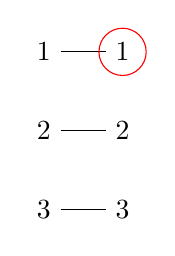
\begin{tikzpicture}
  \graph {
    { [name=first]  1, 2, 3} --
    { [name=second] 1, 2, 3}
  };
  \draw [red] (second 1) circle [radius=3mm];
\end{tikzpicture}
\end{codeexample}
            %
            Note that, indeed, in the above example six nodes are created even
            though the first and second set of nodes have the same \meta{node
            name}. The reason is that the full names of the six nodes are all
            different. Also note that only the \meta{node name} is used as the
            node text, not the full name. This can be changed as described
            later on.

            This key can be used repeatedly, leading to ever longer node names.
        \end{key}

        \begin{key}{/tikz/graphs/name separator=\meta{symbols} (initially \string\space)}
            Changes the symbol that is used to separate the \meta{text} from
            the \meta{node name}. The default is |\space|, resulting in a
            space.
            %
\begin{codeexample}[]
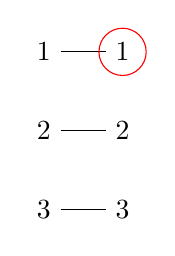
\begin{tikzpicture}
  \graph [name separator=] { % no separator
    { [name=first]  1, 2, 3} --
    { [name=second] 1, 2, 3}
  };
  \draw [red] (second1) circle [radius=3mm];
\end{tikzpicture}
\end{codeexample}
            %
\begin{codeexample}[]
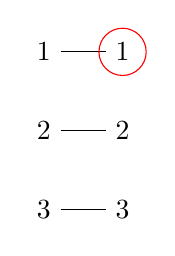
\begin{tikzpicture}
  \graph [name separator=-] {
    { [name=first]  1, 2, 3} --
    { [name=second] 1, 2, 3}
  };
  \draw [red] (second-1) circle [radius=3mm];
\end{tikzpicture}
\end{codeexample}
        \end{key}
    \item The \meta{node options} are
        %
        \begin{enumerate}
            \item The options that have accumulated in calls to |nodes| from
                the surrounding scopes.
            \item The local \meta{options}.
        \end{enumerate}
        %
        The options are executed with the path prefix |/tikz/graphs|, but any
        unknown key is executed with the prefix |/tikz|. This means, in
        essence, that some esoteric keys are more difficult to use inside the
        options and that any key with the prefix |/tikz/graphs| will take
        precedence over a key with the prefix |/tikz|.
    \item The \meta{text} that is passed to the |\node| command is computed as
        follows: First, you can use the following key to directly set the
        \meta{text}:
        %
        \begin{key}{/tikz/graphs/as=\meta{text}}
            The \meta{text} is used as the text of the node. This allows you to
            provide a text for the node that differs arbitrarily from the name
            of the node.
            %
\begin{codeexample}[]
\tikz \graph { a [as=$x$] -- b [as=$y_5$] -> c [red, as={a--b}] };
\end{codeexample}
            %
            This key always takes precedence over all of the mechanisms
            described below.
        \end{key}
        %
        In case the |as| key is not used, a default text is chosen as follows:
        First, when a direct node specification contains a slash (or, for
        historical reasons, a double underscore), the text to the right of the
        slash (or double underscore) is stored in the macro
        |\tikzgraphnodetext|; if there is no slash, the \meta{node name} is
        stored in |\tikzgraphnodetext|, instead. Then, the current value of the
        following key is used as \meta{text}:
        %
        \begin{key}{/tikz/graphs/typeset=\meta{code}}
            The macro or code stored in this key is used as the \meta{text} if
            the node. Inside the \meta{code}, the following macros are
            available:
            %
            \begin{command}{\tikzgraphnodetext}
                This macro expands to the \meta{text} to the right of the
                double underscore or slash in a direct node specification or,
                if there is no slash, to the \meta{node name}.
            \end{command}
            %
            \begin{command}{\tikzgraphnodename}
                This macro expands to the name of the current node without the
                path.
            \end{command}
            %
            \begin{command}{\tikzgraphnodepath}
                This macro expands to the current path of the node. These paths
                result from the use of the |name| key as described above.
            \end{command}
            %
            \begin{command}{\tikzgraphnodefullname}
                This macro contains the concatenation of the above two.
            \end{command}
        \end{key}
        %
        By default, the typesetter is just set to |\tikzgraphnodetext|, which
        means that the default text of a node is its name. However, it may be
        useful to change this: For instance, you might wish that the text of
        all graph nodes is, say, surrounded by parentheses:
        %
\begin{codeexample}[]
\tikz \graph [typeset=(\tikzgraphnodetext)]
  { a -> b -> c };
\end{codeexample}
        %
        A more advanced macro might take apart the node text and render it
        differently:
        %
\begin{codeexample}[]
\def\mytypesetter{\expandafter\myparser\tikzgraphnodetext\relax}
\def\myparser#1 #2 #3\relax{%
  $#1_{#2,\dots,#3}$
}
\tikz \graph [typeset=\mytypesetter, grow down]
  { a 1 n -> b 2 m -> c 4 nm };
\end{codeexample}
        %
        The following styles install useful predefined typesetting macros:
        %
        \begin{key}{/tikz/graphs/empty nodes}
            Just sets |typeset| to nothing, which causes all nodes to have an
            empty text (unless, of course, the |as| option is used):
            %
\begin{codeexample}[]
\tikz \graph [empty nodes, nodes={circle, draw}] { a -> {b, c} };
\end{codeexample}
        \end{key}
        %
        \begin{key}{/tikz/graphs/math nodes}
            Sets |typeset| to |$\tikzgraphnodetext$|, which causes all nodes
            names to be typeset in math mode:
            %
\begin{codeexample}[]
\tikz \graph [math nodes, nodes={circle, draw}] { a_1 -> {b^2, c_3^n} };
\end{codeexample}
        \end{key}
\end{itemize}

If a node is referenced instead of fresh, then this node becomes the node that
will be connected by the preceding or following edge specification to other
nodes. The \meta{options} are executed even for a referenced node, but they
cannot be used to change the appearance of the node (because the node exists
already). Rather, the \meta{options} can only be used to change the logical
coloring of the node, see Section~\ref{section-library-graphs-color-classes}
for details.

\medskip
\textbf{Quoted Node Names.} When the \meta{node name} and/or the \meta{text} of
a node is surrounded by quotation marks, you can use all sorts of special
symbols as part of the text that are normally forbidden:
%
\begin{codeexample}[]
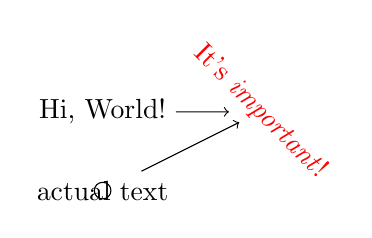
\begin{tikzpicture}
  \graph [grow right=2cm] {
    "Hi, World!"       -> "It's \emph{important}!"[red,rotate=-45];
    "name"/actual text -> "It's \emph{important}!";
  };
  \draw (name) circle [radius=3pt];
\end{tikzpicture}
\end{codeexample}

In detail, for the following happens when quotation marks are encountered at
the beginning of a node name or its text:
%
\begin{itemize}
    \item Everything following the quotation mark up to the next single
        quotation mark is collected into a macro \meta{collected}. All sorts of
        special characters, including commas, square brackets, dashes, and even
        backslashes are allowed here. Basically, the only restriction is that
        braces must be balanced.
    \item A double quotation mark (|""|) does not count as the ``next single
        quotation mark''. Rather, it is replaced by a single quotation mark.
        For instance, |"He said, ""Hello world."""| would be stored inside
        \meta{collected} as |He said, "Hello world."| However, this rule
        applies only on the outer-most level of braces. Thus, in
        %
\begin{codeexample}[code only]
"He {said, ""Hello world.""}"
\end{codeexample}
        %
        we would get |He {said, ""Hello world.""}| as \meta{collected}.
    \item ``The next single quotation mark'' refers to the next quotation mark
        on the current level of braces, so in |"hello {"} world"|, the next
        quotation mark would be the one following |world|.
\end{itemize}

Now, once the \meta{collected} text has been gather, it is used as follows:
When used as \meta{text} (what is actually displayed), it is just used ``as
is''. When it is used as \meta{node name}, however, the following happens:
Every ``special character'' in \meta{collected} is replaced by its Unicode
name, surrounded by |@|-signs. For instance, if \meta{collected} is
|Hello, world!|, the \meta{node name} is the somewhat longer text
|Hello@COMMA@ world@EXCLAMATION MARK@|. Admittedly, referencing such a node
from outside the graph is cumbersome, but when you use exactly the same
\meta{collected} text once more, the same \meta{node name} will result. The
following characters are considered ``special'':
%
\begin{quote}
    \texttt{\char`\|}|$&^~_[](){}/.-,+*'`!":;<=>?@#%\{}|%$
\end{quote}
%
These are exactly the Unicode character with a decimal code number between 33
and 126 that are neither digits nor letters.

\medskip
\textbf{Reference Node Specifications.} A reference node specification is a
node specification that starts with an opening parenthesis. In this case,
parentheses must surround a \meta{name} as in |(foo)|, where |foo| is the
\meta{name}. The following will now happen:
%
\begin{enumerate}
    \item It is tested whether \meta{name} is the name of a currently active
        \emph{node set}. This case will be discussed in a moment.
    \item Otherwise, the \meta{name} is interpreted and treated as a referenced
        node, but independently of whether the node has already been fresh in
        the current graph or not. In other words, the node must have been
        defined either already inside the graph (in which case the parenthesis
        are more or less superfluous) or it must have been defined outside the
        current picture.

        The way the referenced node is handled is the same way as for a direct
        node that is a referenced node.

        If the node does not already exist, an error message is printed.
\end{enumerate}

Let us now have a look at node sets. Inside a |{tikzpicture}| you can locally
define a \emph{node set} by using the following key:
%
\begin{key}{/tikz/new set=\meta{set name}}
    This will setup a node set named \meta{set name} within the current scope.
    Inside the scope, you can add nodes to the node set using the |set| key. If
    a node set of the same name already exists in the current scope, it will be
    reset and made empty for the current scope.

    Note that this command has the path |/tikz| and is normally used
    \emph{outside} the |graph| command.
\end{key}
%
\begin{key}{/tikz/set=\meta{set name}}
    This key can be used as an option with a |node| command. The \meta{set
    name} must be the name of a node set that has previously been created
    inside some enclosing scope via the |new set| key. The effect is that the
    current node is added to the node set.
\end{key}

When you use a |graph| command inside a scope where some node set called
\meta{set name} is defined, then inside this |graph| command you use
|(|\meta{set name}|)| to reference \emph{all} of the nodes in the node set. The
effect is the same as if instead of the reference to the set name you had
created a group specification containing a list of references to all the nodes
that are part of the node set.
%
\begin{codeexample}[]
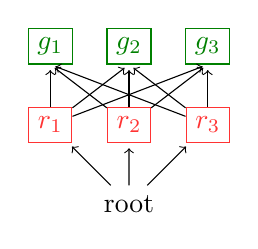
\begin{tikzpicture}[new set=red, new set=green, shorten >=2pt]
  \foreach \i in {1,2,3} {
    \node [draw, red!80,         set=red]   (r\i) at (\i,1) {$r_\i$};
    \node [draw, green!50!black, set=green] (g\i) at (\i,2) {$g_\i$};
  }
  \graph {
    root [xshift=2cm] ->
    (red)             -> [complete bipartite, right anchor=south]
    (green)
  };
\end{tikzpicture}
\end{codeexample}

There is an interesting caveat with referencing node sets: Suppose that at the
beginning of a graph you just say |(foo);| where |foo| is a set name. Unless
you have specified special options, this will cause the following to happen: A
group is created whose members are all the nodes of the node set |foo|. These
nodes become referenced nodes, but otherwise nothing happens since, by default,
the nodes of a group are not connected automatically. However, the referenced
nodes have now been referenced inside the graph, you can thus subsequently
access them as if they had been defined inside the graph. Here is an example
showing how you can create nodes outside a |graph| command and then connect
them inside as if they had been declared inside:
%
\begin{codeexample}[]
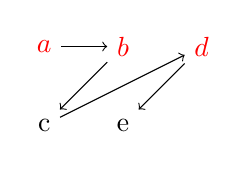
\begin{tikzpicture}[new set=import nodes]
  \begin{scope}[nodes={set=import nodes}] % make all nodes part of this set
    \node [red] (a) at (0,1) {$a$};
    \node [red] (b) at (1,1) {$b$};
    \node [red] (d) at (2,1) {$d$};
  \end{scope}

  \graph {
    (import nodes);         % "import" the nodes

    a -> b -> c -> d -> e;  % only c and e are new
  };
\end{tikzpicture}
\end{codeexample}

\medskip
\textbf{Group Node Specifications.} At a place where a node specification
should go, you can also instead provide a group specification. Since nodes
specifications are part of chain specifications, which in turn are part of
group specifications, this is a recursive definition.
%
\begin{codeexample}[]
\tikz \graph { a -> {b,c,d} -> {e -> {f,g}, h} };
\end{codeexample}

As can be seen in the above example, when two groups of nodes are connected via
an edge specification, it is not immediately obvious which connecting edges are
added. This is detailed in Section~\ref{section-library-graphs-color-classes}.


\subsubsection{Specifying Tries}

In computer science, a \emph{trie} is a special kind of tree, where for each
node and each symbol of an alphabet, there is at most one child of the node
labeled with this symbol.

The |trie| key is useful for drawing tries, but it can also be used in other
situations. What it does, essentially, is to prepend the node names of all
nodes \emph{before} the current node of the current chain to the node's name.
This will often make it easier or more natural to specify graphs in which
several nodes have the same label.

\begin{key}{/tikz/graphs/trie=\opt{\meta{true or false}} (default true, initially false)}
    If this key is set to |true|, after a node has been created on a chain, the
    |name| key is executed with the node's \meta{node name}. Thus, all nodes
    later on this chain have the ``path'' of nodes leading to this node as
    their name. This means, in particular, that
    %
    \begin{enumerate}
        \item two nodes of the same name but in different parts of a chain will
            be different,
        \item while if another chain starts with the same nodes, no new nodes
            get created.
    \end{enumerate}
    %
    In total, this is exactly the behaviour you would expect of a trie:
    %
\begin{codeexample}[]
\tikz \graph [trie] {
  a -> {
    a,
    c -> {a, b},
    b
  }
};
\end{codeexample}
    %
    You can even ``reiterate'' over a path in conjunction with the |simple|
    option. However, in this case, the default placement strategies will not
    work and you will need options like |layered layout| from the graph drawing
    libraries, which need Lua\TeX.
    %
\ifluatex
\begin{codeexample}[preamble={\usetikzlibrary{graphdrawing}\usegdlibrary{layered}}]
\tikz \graph [trie, simple, layered layout] {
  a -> b -> a,
  a -> b -> c,
  a -> {d,a}
};
\end{codeexample}
    %
    In the following example, we setup the |typeset| key so that it shows the
    complete names of the nodes:
    %
\begin{codeexample}[preamble={\usetikzlibrary{graphdrawing}\usegdlibrary{layered}}]
\tikz \graph [trie, simple, layered layout,
              typeset=\tikzgraphnodefullname] {
  a -> b -> a,
  a -> b -> c,
  a -> {d,a}
};
\end{codeexample}
\fi
    %
    You can also use the |trie| key locally and later reference nodes using
    their full name:
    %
\begin{codeexample}[]
\tikz \graph {
  { [trie, simple]
    a -> {
      b,
      c -> a
    }
  },
  a b ->[red] a c a
};
\end{codeexample}
    %
\end{key}


\subsection{Quick Graphs}
\label{section-library-graphs-quick}

The graph syntax is powerful, but this power comes at a price: parsing the
graph syntax, which is done by \TeX, can take some time. Normally, the parsing
is fast enough that you will not notice it, but it can be bothersome when you
have graphs with hundreds of nodes as happens frequently when nodes are
generated algorithmically by some other program. Fortunately, when another
program generated a graph specification, we typically do not need the full
power of the graph syntax. Rather, a small subset of the graph syntax would
suffice that allows to specify nodes and edges. For these reasons, the is a
special ``quick'' version of the graph syntax.

Note, however, that using this syntax will usually at most halve the time
needed to parse a graph. Thus, it really mostly makes sense in conjunction with
large, algorithmically generated graphs.

\begin{key}{/tikz/graphs/quick}
    When you provide this key with a graph, the syntax of graph specifications
    gets restricted. You are no longer allowed to use certain features of the
    graph syntax; but all features that are still allowed are also allowed in
    the same way when you do not provide the |quick| option. Thus, leaving out
    the |quick| option will never hurt.

    Since the syntax is so severely restricted, it is easier to explain which
    aspects of the graph syntax \emph{will} still work:
    %
    \begin{enumerate}
        \item A quick graph consists of a sequence of either nodes, edges
            sequences, or groups. These are separated by commas or semicolons.
        \item Every node is of the form
            %
            \begin{quote}
                |"|\meta{node name}|"|\opt{|/"|\meta{node text}|"[|\meta{options}|]|}
            \end{quote}

            The quotation marks are mandatory. The part |/"|\meta{node text}|"|
            may  be missing, in which case the node name is used as the node
            text. The \meta{options} may also be missing. The \meta{node name}
            may not contain any ``funny'' characters (unlike in the normal
            graph command).
        \item Every chain is of the form
            %
            \begin{quote}
                \meta{node spec} \meta{connector} \meta{node spec}
                \meta{connector} \dots \meta{connector} \meta{node spec}|;|
            \end{quote}

            Here, the \meta{node spec} are node specifications as described
            above, the \meta{connector} is one of the four connectors |->|,
            |<-|, |--|, and |<->| (the connector |-!-| is not allowed since the
            |simple| option is also not allowed). Each connector may be
            followed by options in square brackets. The semicolon may be
            replaced by a comma.
        \item Every group is of the form
            %
            \begin{quote}
                |{ [|\meta{options}|]| \meta{chains and groups} |};|
            \end{quote}
            %
            The \meta{options} are compulsory. The semicolon can, again, be
            replaced by a comma.
        \item The |number nodes| option will work as expected.
    \end{enumerate}

    Here is a typical way this syntax might be used:
    %
\begin{codeexample}[preamble={\usetikzlibrary{quotes}}]
\tikz \graph [quick] { "a" --["foo"] "b"[x=1] };
\end{codeexample}

\begin{codeexample}[]
\tikz \graph [quick] {
  "a"/"$a$" -- "b"[x=1] --[red] "c"[x=2];
  { [nodes=blue] "a" -- "d"[y=1]; };
};
\end{codeexample}

    Let us now have a look at the most important things that will \emph{not}
    work when the |quick| option is used:

    \begin{itemize}
        \item Connecting a node and a group as in |a->{b,c}|.
        \item Node names without quotation marks as in |a--b|.
        \item Everything described in subsequent subsections, which includes
            subgraphs (graph macros), graph sets, graph color classes,
            anonymous nodes, the |fresh nodes| option, sublayouts, simple
            graphs, edge annotations.
        \item Placement strategies -- you either have to define all node
            positions explicitly using |at=| or |x=| and |y=| or you must use a
            graph drawing algorithm like |layered layout|.
    \end{itemize}
\end{key}


\subsection{Simple Versus Multi-Graphs}
\label{section-library-graphs-simple}

The |graphs| library allows you to construct both simple graphs and
multi-graphs. In a simple graph there can be at most one edge between any two
vertices, while in a multi-graph there can be multiple edges (hence the name).
The two keys |multi| and |simple| allow you to switch (even locally inside on
of the graph's scopes) between which kind of graph is being constructed. By
default, the |graph| command produces a multi-graph since these are faster to
construct.

\begin{key}{/tikz/graphs/multi}
    When this edge is set for a whole graph (which is the default) or just for
    a group (which is useful if the whole graph is simple in general, but a
    part is a multi-graph), then when you specify an edge between two nodes
    several times, several such edges get created:
    %
\begin{codeexample}[]
\tikz \graph [multi] { % "multi" is not really necessary here
  a ->[bend left,  red]  b;
  a ->[bend right, blue] b;
};
\end{codeexample}
    %
    In case |multi| is used for a scope inside a larger scope where the
    |simple| option is specified, then inside the local |multi| scope edges are
    immediately created and they are completely ignored when it comes to
    deciding which kind of edges should be present in the surrounding simple
    graph. From the surrounding scope's point of view it is as if the local
    |multi| graph contained no edges at all.

    This means, in particular, that you can use the |multi| option with a
    single edge to ``enforce'' this edge to be present in a simple graph.
\end{key}

\begin{key}{/tikz/graphs/simple}
    In contrast a multi-graph, in a simple graph, at most one edge gets created
    for every pair of vertices:
    %
\begin{codeexample}[]
\tikz \graph [simple]{
  a ->[bend left,  red]  b;
  a ->[bend right, blue] b;
};
\end{codeexample}
    %
    As can be seen, the second edge ``wins'' over the first edge. The general
    rule is as follows: In a simple graph, whenever an edge between two
    vertices is specified multiple times, only the very last specification and
    its options will actually be executed.

    The real power of the |simple| option lies in the fact that you can first
    create a complicated graph and then later redirect and otherwise modify
    edges easily:
    %
\begin{codeexample}[]
\tikz \graph [simple, grow right=2cm] {
  {a,b,c,d} ->[complete bipartite] {e,f,g,h};

  { [edges={red,thick}] a -> e -> d -> g -> a };
};
\end{codeexample}

    One particularly interesting kind of edge specification for a simple graph
    is |-!-|. Recall that this is used to indicate that ``no edge'' should be
    added between certain nodes. In a multi-graph, this key usually has no
    effect (unless the key |new -!-| has been redefined) and is pretty
    superfluous. In a simple graph, however, it counts as an edge kind and you
    can thus use it to remove an edge that been added previously:
    %
\begin{codeexample}[preamble={\usetikzlibrary{graphs.standard}}]
\tikz \graph [simple] {
  subgraph K_n [n=8, clockwise];
  % Get rid of the following edges:
  1 -!- 2;
  3 -!- 4;
  6 -!- 8;
  % And make one edge red:
  1 --[red] 3;
};
\end{codeexample}

    Creating a graph such as the above in other fashions is pretty awkward.

    For every unordered pair $\{u,v\}$ of vertices at most one edge will be
    created in a simple graph. In particular, when you say |a -> b| and later
    also |a <- b|, then only the edge |a <- b| will be created. Similarly, when
    you say |a -> b| and later |b -> a|, then only the edge |b -> a| will be
    created.

    The power of the |simple| command comes at a certain cost: As the graph is
    being constructed, a (sparse) array is created that keeps track for each
    edge of the last edge being specified. Then, at the end of the scope
    containing the |simple| command, for every pair of vertices the edge is
    created. This is implemented by two nested loops iterating over all
    possible pairs of vertices -- which may take quite a while in a graph of,
    say, 1000 vertices. Internally, the |simple| command is implemented as an
    operator that adds the edges when it is called, but this should be
    unimportant in normal situations.
\end{key}


\subsection{Graph Edges: Labeling and Styling}

When the |graphs| library creates an edge between two nodes in a graph, the
appearance (called ``styling'' in \tikzname) can be specified in different
ways. Sometimes you will simply wish to say ``the edges between these two
groups of node should be red'', but sometimes you may wish to say ``this
particular edge going into this node should be red''. In the following,
different ways of specifying such styling requirements are discussed. Note that
adding labels to edges is, from \tikzname's point of view, almost the same as
styling edges, since they are also specified using options.


\subsubsection{Options For All Edges Between Two Groups}

When you write |... ->[options] ...| somewhere inside your graph specification,
this typically cause one or more edges to be created between the nodes in the
chain group before the |->| and the nodes in the chain group following it. The
|options| are applied to all of them. In particular, if you use the |quotes|
library and you write some text in quotes inside the |options|, this text will
be added as a label to each edge:
%
\begin{codeexample}[preamble={\usetikzlibrary{quotes}}]
\tikz
  \graph [edge quotes=near start] {
    { a, b } -> [red, "x", complete bipartite] { c, d };
  };
\end{codeexample}

As documented in the |quotes| library in more detail, you can easily modify the
appearance of edge labels created using the quotes syntax by adding options
after the closing quotes:
%
\begin{codeexample}[preamble={\usetikzlibrary{quotes}}]
\tikz \graph {
  a ->["x"] b ->["y"'] c ->["z" red] d;
};
\end{codeexample}

The following options make it easy to setup the styling of nodes created in
this way:
%
\begin{key}{/tikz/graphs/edge quotes=\opt{\meta{options}}}
    A shorthand for setting the style |every edge quotes| to \meta{options}.
    %
\begin{codeexample}[preamble={\usetikzlibrary{quotes}}]
  \tikz \graph [edge quotes={blue,auto}] {
  a ->["x"] b ->["y"'] c ->["b" red] d;
};
\end{codeexample}
    %
\end{key}

\begin{key}{/tikz/graphs/edge quotes center}
    A shorthand for |edge quotes| to |anchor=center|.
    %
\begin{codeexample}[preamble={\usetikzlibrary{quotes}}]
\tikz \graph [edge quotes center] {
  a ->["x"] b ->["y"] c ->["z" red] d;
};
\end{codeexample}
    %
\end{key}

\begin{key}{/tikz/graphs/edge quotes mid}
    A shorthand for |edge quotes| to |anchor=mid|.
    %
\begin{codeexample}[preamble={\usetikzlibrary{quotes}}]
\tikz \graph [edge quotes mid] {
  a ->["x"] b ->["y"] c ->["z" red] d;
};
\end{codeexample}
    %
\end{key}


\subsubsection{Changing Options For Certain Edges}

Consider the following tree-like graph:
%
\begin{codeexample}[]
\tikz \graph { a -> {b,c} };
\end{codeexample}

Suppose we wish to specify that the edge from |a| to |b| should be red, while
the edge from |a| to |c| should be blue. The difficulty lies in the fact that
\emph{both} edges are created by the single |->| operator and we can only add
one of these option |red| or |blue| to the operator.

There are several ways to solve this problem. First, we can simply split up the
specification and specify the two edges separately:
%
\begin{codeexample}[]
\tikz \graph {
  a -> [red]  b;
  a -> [blue] c;
};
\end{codeexample}
%
While this works quite well, we can no longer use the nice chain group syntax
of the |graphs| library. For the rather simple graph |a->{b,c}| this is not a
big problem, but if you specify a tree with, say, 30 nodes it is really
worthwhile being able to specify the tree ``in its natural form in the \TeX\
code'' rather than having to list all of the edges explicitly. Also, as can be
seen in the above example, the node placement is changed, which is not always
desirable.

One can sidestep this problem using the |simple| option: This option allows you
to first specify a graph and then, later on, replace edges by other edges and,
thereby, provide new options:
%
\begin{codeexample}[]
\tikz \graph [simple] {
  a -> {b,c};
  a -> [red]  b;
  a -> [blue] c;
};
\end{codeexample}

The first line is the original specification of the tree, while the following
two lines replace some edges of the tree (in this case, all of them) by edges
with special options. While this method is slower and in the above example
creates even longer code, it is very useful if you wish to, say, highlight a
path in a larger tree: First specify the tree normally and, then, ``respecify''
the path or paths with some other edge options in force. In the following
example, we use this to highlight a whole subtree of a larger tree:
    %
\begin{codeexample}[]
\tikz \graph [simple] {
  % The larger tree, no special options in force
  a -> {
    b -> {c,d},
    e -> {f,g},
    h
  },
  { [edges=red] % Now highlight a part of the tree
    a -> e -> {f,g}
  }
};
\end{codeexample}


\subsubsection{Options For Incoming and Outgoing Edges}

When you use the syntax |... ->[options] ...| to specify options, you specify
options for the ``connections between two sets of nodes''. In many cases,
however, it will be more natural to specify options ``for the edges lead to or
coming from a certain node'' and you will want to specify these options ``at
the node''. Returning to the example of the graph |a->{b,c}| where we want a
red edge between |a| and |b| and a blue edge between |a| and |c|, this could
also be phrased as follows: ``Make the edge leading to |b| red and make the
edge leading to |c| blue''.

For this situation, the |graphs| library offers a number of special keys, which
are documented in the following. However, most of the time you will not use
these keys directly, but, rather, use a special syntax explained in
Section~\ref{section-syntax-outgoing-incoming}.

\begin{key}{/tikz/graphs/target edge style=\meta{options}}
    This key can (only) be used with a \emph{node} inside a graph
    specification. When used, the \meta{options} will be added to every edge
    that is created by a connector like |->| in which the node is a
    \emph{target}. Consider the following example:
    %
\begin{codeexample}[]
\tikz \graph {
  { a, b } ->
  { c [target edge style=red], d } ->
  { e, f }
};
\end{codeexample}
    %
    In the example, only when the edge from |a| to |c| is created, |c| is the
    ``target'' of the edge. Thus, only this edge becomes red.

    When an edge already has options set directly, the \meta{options} are
    executed after these direct options, thus, they ``overrule'' them:
    %
\begin{codeexample}[]
\tikz \graph {
  { a, b } -> [blue, thick]
  { c [target edge style=red], d } ->
  { e, f }
};
\end{codeexample}

    The \meta{options} set in this way will stay attached to the node, so also
    for edges created later on that lead to the node will have these options
    set:
    %
\begin{codeexample}[]
\tikz \graph {
  { a, b } ->
  { c [target edge style=red], d } ->
  { e, f },
  b -> c
};
\end{codeexample}

    Multiple uses of this key accumulate. However, you may sometimes also wish
    to ``clear'' these options for a key since at some later point you no
    longer wish the \meta{options} to be added when some further edges are
    added. This can be achieved using the following key:
    %
    \begin{key}{/tikz/graphs/target edge clear}
        Clears all \meta{options} for edges with the node as a target and
        also edge labels (see below) for this node.
    \end{key}
    %
\begin{codeexample}[]
\tikz \graph {
  { a, b } ->
  { c [target edge style=red], d },
  b -> c[target edge clear]
};
\end{codeexample}
    %
\end{key}

\begin{key}{/tikz/graphs/target edge node=\meta{node specification}}
    This key works like |target edge style|, only the \meta{node specification}
    will not be added as options to any newly created edges with the current
    node as their target, but rather it will be added as a node specification.
    %
\begin{codeexample}[]
\tikz \graph {
  { a, b } ->
  { c [target edge node=node{X}], d } ->
  { e, f }
};
\end{codeexample}
    %
    As for |target edge style| multiple uses of this key accumulate and the key
    |target edge clear| will (also) clear all target edge nodes that have been
    set for a node earlier on.
\end{key}

\begin{key}{/tikz/graphs/source edge style=\meta{options}}
    Works exactly like |target edge style|, only now the \meta{options} are
    only added when the node is a source of a newly created edge:
    %
\begin{codeexample}[]
\tikz \graph {
  { a, b } ->
  { c [source edge style=red], d } ->
  { e, f }
};
\end{codeexample}
    %
    If both for the source and also for the target of an edge \meta{options}
    have been specified, the options are applied in the following order:
    %
    \begin{enumerate}
        \item First come the options from the edge itself.
        \item Then come the options contributed by the source node using this
            key.
        \item Then come the options contributed by the target node using
            |target node style|.
    \end{enumerate}
    %
\begin{codeexample}[]
\tikz \graph {
  a [source edge style=red] ->[green]
  b [target edge style=blue]  % blue wins
};
\end{codeexample}
    %
\end{key}

\begin{key}{/tikz/graphs/source edge node=\meta{node specification}}
    Works like |source edge style| and |target edge node|.
\end{key}

\begin{key}{/tikz/graphs/source edge clear=\meta{node specification}}
    Works like |target edge clear|.
\end{key}


\subsubsection{Special Syntax for Options For Incoming and Outgoing Edges}
\label{section-syntax-outgoing-incoming}

The keys |target node style| and its friends are powerful, but a bit cumbersome
to write down. For this reason, the |graphs| library introduces a special
syntax that is based on what I call the ``first-char syntax'' of keys. Inside
the options of a node inside a graph, the following special rules apply:
%
\begin{enumerate}
    \item Whenever an option starts with |>|, the rest of the options are
        passed to |target edge style|. For instance, when you write |a[>red]|,
        then this has the same effect as if you had written
        %
\begin{codeexample}[code only]
a[target edge style={red}]
\end{codeexample}
        %
    \item Whenever an options starts with |<|, the rest of the options are
        passed to |source edge style|.
    \item In both of the above case, in case the options following the |>| or
        |<| sign start with a quote, the created edge label is passed to
        |source edge node| or |target edge node|, respectively.

        This is exactly what you want to happen.
\end{enumerate}
%
Additionally, the following styles provide shorthands for ``clearing'' the
target and source options:
%
\begin{key}{/tikz/graphs/clear >}
    A more easy-to-remember shorthand for |target edge clear|.
\end{key}
%
\begin{key}{/tikz/graphs/clear <}
    A more easy-to-remember shorthand for |source edge clear|.
\end{key}

These mechanisms make it especially easy to create trees in which the edges are
labeled in some special way:
%
\begin{codeexample}[preamble={\usetikzlibrary{quotes}}]
\tikz
  \graph [edge quotes={fill=white,inner sep=1pt},
          grow down, branch right] {
    / -> h [>"9"] -> {
      c [>"4" text=red,] -> {
        a [>"2", >thick],
        e [>"0"]
      },
      j [>"7"]
    }
  };
\end{codeexample}


\subsubsection{Placing Node Texts on Incoming Edges}

Normally, the text of a node is shown (only) inside the node. In some case, for
instance when drawing certain kind of trees, the nodes themselves should not
get any text, but rather the edge leading to the node should be labeled as in
the following example:
%
\begin{codeexample}[preamble={\usetikzlibrary{quotes}}]
\tikz \graph [empty nodes]
{
  root -> {
    a [>"a"],
    b [>"b"] -> {
      c [>"c"],
      d [>"d"]
    }
  }
};
\end{codeexample}
%
As the example shows, it is a bit cumbersome that we have to label the nodes
and then specify the same text once more using the incoming edge syntax.

For these cases, it would be better if the text of the node where not used with
the node but, rather, be passed directly to the incoming or the outgoing edge.
The following styles do exactly this:

\begin{key}{/tikz/graphs/put node text on incoming edges=\opt{\meta{options}}}
    When this key is used with a node or a group, the following happens:
    %
    \begin{enumerate}
        \item The command
            |target edge node={node[|\meta{options}|]{\tikzgraphnodetext}}| is
            executed. This means that all incoming edges of the node get a
            label with the text that would usually be displayed in the node.
            You can use keys like |math nodes| normally.
        \item The command |as={}| is executed. This means that the node itself
            will display nothing.
    \end{enumerate}
    %
    Here is an example that show how this command is used.
    %
\begin{codeexample}[]
\tikz \graph [put node text on incoming edges,
              math nodes, nodes={circle,draw}]
  { a -> b -> {c, d} };
\end{codeexample}
    %
\end{key}

\begin{key}{/tikz/graphs/put node text on outgoing edges=\opt{\meta{options}}}
    Works like the previous key, only with |target| replaced by |source|.
\end{key}


\subsection{Graph Operators, Color Classes, and Graph Expressions}
\label{section-library-graphs-color-classes}

\tikzname's |graph| command employs a powerful mechanism for adding edges
between nodes and sets of nodes. To a graph theorist, this mechanism may be
known as a \emph{graph expression}: A graph is specified by starting with small
graphs and then applying \emph{operators} to them that form larger graphs and
that connect and recolor colored subsets of the graph's node in different ways.


\subsubsection{Color Classes}
\label{section-library-graph-coloring}

\tikzname\ keeps track of a \emph{(multi)coloring} of the graph as it is being
constructed. This does not mean that the actual color of the nodes on the page
will be different, rather, in the following we refer to ``logical'' colors in
the way graph theoreticians do. These ``logical'' colors are only important
while the graph is being constructed and they are ``thrown away'' at the end of
the construction. The actual (``physical'') colors of the nodes are set
independently of these logical colors.

As a graph is being constructed, each node can be part of one or more
overlapping \emph{color classes}. So, unlike what is sometimes called a
\emph{legal coloring}, the logical colorings that \tikzname\ keeps track of may
assign multiple colors to the same node and two nodes connected by an edge may
well have the same color.

Color classes must be declared prior to use. This is done using the following
key:
%
\begin{key}{/tikz/graphs/color class=\meta{color class name}}
    This sets up a new color class called \meta{color class name}. Nodes and
    whole groups of nodes can now be colored with \meta{color class name}. This
    is done using the following keys, which become
    available inside the current scope:
    %
    \begin{key}{/tikz/graphs/\meta{color class name}}
        This key internally uses the |operator| command to setup an operator
        that will cause all nodes of the current group to get the ``logical
        color'' \meta{color class name}. Nodes retain this color in all
        encompassing scopes, unless it is explicitly changed (see below) or
        unset (again, see below).
        %
\begin{codeexample}[]
\tikz \graph [color class=red] {
  [cycle=red]  % causes all "logically" red nodes to be connected in
               % a cycle
  a,
  b [red],
  { [red] c ->[bend right] d },
  e
};
\end{codeexample}
        %
\begin{codeexample}[]
\tikz \graph [color class=red, color class=green,
              math nodes, clockwise, n=5] {
  [complete bipartite={red}{green}]
  { [red]   r_1, r_2 },
  { [green] g_1, g_2, g_3 }
};
\end{codeexample}
    \end{key}
    %
    \begin{key}{/tikz/graphs/not \meta{color class name}}
        Sets up an operator for the current scope so that all nodes in it loose
        the color \meta{color class name}. You can also use |!|\meta{color
        class name} as an alias for this key.
        %
\begin{codeexample}[]
\tikz \graph [color class=red, color class=green,
              math nodes, clockwise, n=5] {
  [complete bipartite={red}{green}]
  { [red]   r_1, r_2 },
  { [green] g_1, g_2, g_3 },
  g_2 [not green]
};
\end{codeexample}
    \end{key}
    %
    \begin{key}{/tikz/graphs/recolor \meta{color class name} by=\meta{new color}}
        Causes all keys having color \meta{color class name} to get \meta{new
        color} instead. They loose having color \meta{color class name}, but
        other colors are not affected.
        %
\begin{codeexample}[]
\tikz \graph [color class=red, color class=green,
              math nodes, clockwise, n=5] {
  [complete bipartite={red}{green}]
  { [red]   r_1, r_2 },
  { [green] g_1, g_2, g_3 },
  g_2 [recolor green by=red]
};
\end{codeexample}
    \end{key}
\end{key}

The following color classes are available by default:
%
\begin{itemize}
    \item Color class |all|. Every node is part of this class by default. This
        is useful to access all nodes of a (sub)graph, since you can simply
        access all nodes of this color class.
    \item Color classes |source| and |target|. These classes are used to
        identify nodes that lead ``into'' a group of nodes and nodes from which
        paths should ``leave'' the group. Details on how these colors are
        assigned are explained in Section~\ref{section-library-graphs-join}. By
        saying |not source| or |not target| with a node, you can influence how
        it is connected:
        %
\begin{codeexample}[]
\tikz \graph { a -> { b, c, d } -> e };
  \end{codeexample}
  \begin{codeexample}[]
\tikz \graph { a -> { b[not source], c, d[not target] } -> e };
  \end{codeexample}
        %
    \item Color classes |source'| and |target'|. These are temporary colors
        that are also explained in Section~\ref{section-library-graphs-join}.
\end{itemize}


\subsubsection{Graph Operators on Groups of Nodes}

Recall that the |graph| command constructs graphs recursively from nested
\meta{group specifications}. Each such \meta{group specification} describes a
subset of the nodes of the final graph. A \emph{graph operator} is an algorithm
that gets the nodes of a group as input and (typically) adds edges between
these nodes in some sensible way. For instance, the |clique| operator will
simply add edges between all nodes of the group.

\begin{key}{/tikz/graphs/operator=\meta{code}}
    This key has an effect in three places:
    %
    \begin{enumerate}
        \item It can be used in the \meta{options} of a \meta{direct node
            specification}.
        \item It can be used in the \meta{options} of a \meta{group
            specification}.
        \item It can be used in the \meta{options} of an \meta{edge
            specification}.
    \end{enumerate}
    %
    The first case is a special case of the second, since it is treated like a
    group specification containing a single node. The last case is more
    complicated and discussed in the next section. So, let us focus on the
    second case.

    Even though the \meta{options} of a group are given at the beginning of the
    \meta{group specification}, the \meta{code} is only executed when the group
    has been parsed completely and all its nodes have been identified. If you
    use the |operator| multiple times in the \meta{options}, the effect
    accumulates, that is, all code passed to the different calls of |operator|
    gets executed in the order it is encountered.

    The \meta{code} can do ``whatever it wants'', but it will typically add
    edges between certain nodes. You can configure what kind of edges
    (directed, undirected, etc.) are created by using the following keys:
    %
    \begin{key}{/tikz/graphs/default edge kind=\meta{value} (initially -\/-)}
        This key stores one of the five edge kinds |--|, |<-|, |->|, |<->|, and
        |-!-|. When an operator wishes to create a new edge, it should
        typically set
        %
\begin{codeexample}[code only]
\tikzgraphsset{new \pfkeysvalueof{/tikz/graphs/default edge kind}=...}
\end{codeexample}
        %
        While this key can be set explicitly, it may be more convenient to use
        the abbreviating keys listed below. Also, this key is automatically set
        to the current value of \meta{edge specification} when a joining
        operator is called, see the discussion of joining operators in
        Section~\ref{section-library-graphs-join}.
    \end{key}
    %
    \begin{key}{/tikz/graphs/--}
        Sets the |default edge kind| to |--|.
        %
\begin{codeexample}[preamble={\usetikzlibrary{graphs.standard}}]
\tikz \graph { subgraph K_n [--, n=5, clockwise, radius=6mm] };
\end{codeexample}
    \end{key}
    %
    \begin{key}{/tikz/graphs/->}
        Sets the |default edge kind| to |->|.
        %
\begin{codeexample}[preamble={\usetikzlibrary{graphs.standard}}]
\tikz \graph { subgraph K_n [->, n=5, clockwise, radius=6mm] };
\end{codeexample}
    \end{key}
    %
    \begin{key}{/tikz/graphs/<-}
        Sets the |default edge kind| to |<-|.
        %
\begin{codeexample}[preamble={\usetikzlibrary{graphs.standard}}]
\tikz \graph { subgraph K_n [<-, n=5, clockwise, radius=6mm] };
\end{codeexample}
    \end{key}
    %
    \begin{key}{/tikz/graphs/<->}
        Sets the |default edge kind| to |<->|.
        %
\begin{codeexample}[preamble={\usetikzlibrary{graphs.standard}}]
\tikz \graph { subgraph K_n [<->, n=5, clockwise, radius=6mm] };
\end{codeexample}
    \end{key}
    %
    \begin{key}{/tikz/graphs/-\protect\exclamationmarktext-}
        Sets the |default edge kind| to |-!-|.
    \end{key}

    When the \meta{code} of an operator is executed, the following commands can
    be used to find the nodes that should be connected:
    %
    \begin{command}{\tikzgraphforeachcolorednode\marg{color name}\marg{macro}}
        When this command is called inside \meta{code}, the following will
        happen: \tikzname\ will iterate over all nodes inside the
        just-specified group that have the color \meta{color name}. The order
        in which they are iterated over is the order in which they appear
        inside the group specification (if a node is encountered several times
        inside the specification, only the first occurrence counts). Then, for
        each node the \meta{macro} is executed with the node's name as the only
        argument.

        In the following example we use an operator to connect every node
        colored |all| inside the subgroup to he node |root|.
        %
\begin{codeexample}[]
\def\myconnect#1{\tikzset{graphs/new ->={root}{#1}{}{}}}

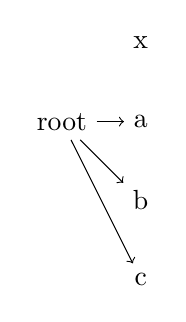
\begin{tikzpicture}
  \node (root) at (-1,-1) {root};

  \graph {
    x,
    {
      [operator=\tikzgraphforeachcolorednode{all}{\myconnect}]
      a, b, c
    }
  };
\end{tikzpicture}
\end{codeexample}
    \end{command}

    \begin{command}{\tikzgraphpreparecolor\marg{color name}\marg{counter}\marg{prefix}}
        This command is used to ``prepare'' the nodes of a certain color for
        random access. The effect is the following: It is counted how many
        nodes there are having color \meta{color name} in the current group and
        the result is stored in \meta{counter}. Next, macros named
        \meta{prefix}|1|, \meta{prefix}|2|, and so on are defined, that store
        the names of the first, second, third, and so on node having the color
        \meta{color name}.

        The net effect is that after you have prepared a color, you can quickly
        iterate over them. This is especially useful when you iterate over
        several color at the same time.

        As an example, let us create an operator then adds a zig-zag path
        between two color classes:
        %
\begin{codeexample}[]
\newcount\leftshorecount   \newcount\rightshorecount
\newcount\mycount          \newcount\myothercount
\def\zigzag{
  \tikzgraphpreparecolor{left shore}\leftshorecount{left shore prefix}
  \tikzgraphpreparecolor{right shore}\rightshorecount{right shore prefix}
  \mycount=0\relax
  \loop
    \advance\mycount by 1\relax%
    % Add the "forward" edge
    \tikzgraphsset{new ->=
      {\csname left shore prefix\the\mycount\endcsname}
      {\csname right shore prefix\the\mycount\endcsname}{}{}}
    \myothercount=\mycount\relax%
    \advance\myothercount by1\relax%
    \tikzgraphsset{new <-=
      {\csname left shore prefix\the\myothercount\endcsname}
      {\csname right shore prefix\the\mycount\endcsname}{}{}}
  \ifnum\myothercount<\leftshorecount\relax
  \repeat
}
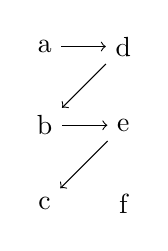
\begin{tikzpicture}
  \graph [color class=left shore, color class=right shore]
  { [operator=\zigzag]
    { [left shore, Cartesian placement]                      a, b, c },
    { [right shore, Cartesian placement, nodes={xshift=1cm}] d, e, f }
  };
\end{tikzpicture}
\end{codeexample}
        %
        Naturally, in order to turn the above code into a usable operator, some
        more code would be needed (like default values and taking care of
        shores of different sizes).
    \end{command}
\end{key}

There are a number of predefined operators, like |clique| or |cycle|, see the
reference Section~\ref{section-library-graphs-reference} for a complete list.


\subsubsection{Graph Operators for Joining Groups}
\label{section-library-graphs-join}

When you join two nodes |foo| and |bar| by the edge specification |->|, it is
fairly obvious, what should happen: An edge from |(foo)| to |(bar)| should be
created. However, suppose we use an edge specification between two node sets
like |{a,b,c}| and |{d,e,f}|. In this case, it is not so clear which edges
should be created. One might argue that all possible edges from any node in the
first set to any node in the second set should be added. On the other hand, one
might also argue that only a matching between these two sets should be created.
Things get even more muddy when a longer chain of node sets are joined.

Instead of fixing how edges are created between two node sets, \tikzname\ takes
a somewhat more general, but also more complicated approach, which can be
broken into two parts. In the following, assume that the following chain
specification is given:
%
\begin{quote}
    \meta{spec$_1$} \meta{edge specification} \meta{spec$_2$}
\end{quote}
%
An example might be |{a,b,c} -> {d, e->f}|.

\medskip
\textbf{The source and target vertices.} Let us start with the question of
which vertices of the first node set should be connected to vertices in the
second node set.

There are two predefined special color classes that are used for this: |source|
and |target|. For every group specification, some vertices are colored as
|source| vertices and some vertices are |target| vertices (a node can both be a
target and a source). Initially, every vertex is both a source and a target,
but that can change as we will see in a moment.

The intuition behind source and target vertices is that, in some sense, edges
``from the outside'' lead into the group via the source vertices and lead out
of the group via the target vertices. To be more precise, the following
happens:
%
\begin{enumerate}
    \item The target vertices of the first group are connected to the source
        vertices of the second group.
    \item In the group resulting from the union of the nodes from
        \meta{spec$_1$} and \meta{spec$_2$}, the source vertices are only those
        from the first group, and the target vertices are only those from the
        second group.
\end{enumerate}

Let us go over the effect of these rules for the example
|{a,b,c} -> {d, e->f}|. First, each individual node is initially both a
|source| and a |target| vertex. Then, in |{a,b,c}| all nodes are still both
source and target vertices since just grouping vertices does not change their
colors. Now, in |e->f| something interesting happens for the first time: the
target vertices of the ``group'' |e| (which is just the node |e|) are connected
to the source vertices of the ``group'' |f|. This means, that an edge is added
from |e| to |f|. Then, in the resulting group |e->f| the only source vertex is
|e| and the only target vertex is |f|. This implies that in the group
|{d,e->f}| the sources are |d| and |e| and the targets are |d| and~|f|.

Now, in |{a,b,c} -> {d,e->f}| the targets  of |{a,b,c}| (which are all three of
them) are connected to the sources of |{d,e->f}| (which are just |d| and~|e|).
Finally, in the whole graph only |a|, |b|, and |c| are sources while only  |d|
and |f| are targets.
%
\begin{codeexample}[]
\def\hilightsource#1{\fill [green, opacity=.25] (#1) circle [radius=2mm]; }
\def\hilighttarget#1{\fill [red,   opacity=.25] (#1) circle [radius=2mm]; }
\tikz \graph
  [operator=\tikzgraphforeachcolorednode{source}{\hilightsource},
   operator=\tikzgraphforeachcolorednode{target}{\hilighttarget}]
  { {a,b,c} -> {d, e->f} };
\end{codeexample}

The next objective is to make more precise what it means that ``the targets of
the first graph'' and the ``sources of the second graph'' should be connected.
We know already of a general way of connecting nodes of a graph: operators!
Thus, we use an operator for this job. For instance, the |complete bipartite|
operator adds an edge from every node having a certain color to every node have
a certain other color. This is exactly what we need here: The first color is
``the color |target| restricted to the nodes of the first graph'' and the
second color is ``the color |source| restricted to the nodes of the second
graph''.

However, we cannot really specify that only nodes from a certain subgraph are
meant -- the |operator| machinery only operates on all nodes of the current
graph. For this reason, what really happens is the following: When the |graph|
command encounters \meta{spec$_1$} \meta{edge specification} \meta{spec$_2$},
it first computes and colors the nodes of the first and the second
specification independently. Then, the |target| nodes of the first graph are
recolored to |target'| and the |source| nodes of the second graph are recolored
to |source'|. Then, the two graphs are united into one graph and a
\emph{joining operator} is executed, which should add edges between |target'|
and |source'|. Once this is done, the colors |target'| and |source'| get
erased. Note that in the resulting graph only the |source| nodes from the first
graph are still |source| nodes and likewise for the |target| nodes of the
second graph.

\medskip
\textbf{The joining operators.} The job of a joining operator is to add edges
between nodes colored |target'| and |source'|. The following rule is used to
determine which operator should be chosen for performing this job:
%
\begin{enumerate}
    \item If the \meta{edge specification} explicitly sets the |operator| key
        to something non-empty (and also not to |\relax|), then the \meta{code}
        of this |operator| call is used.
    \item Otherwise, the current value of the following key is used:
        %
        \begin{key}{/tikz/graphs/default edge operator=\meta{key} (initially matching and star)}
            This key stores the name of a \meta{key} that is executed for every
            \meta{edge specification} whose \meta{options} do not contain the
            |operator| key.
            %
\begin{codeexample}[]
\tikz \graph [default edge operator=matching] {
  {a, b}    ->[matching and star]
  {c, d, e} --[complete bipartite]
  {f, g, h} --
  {i, j, k}
};
\end{codeexample}
        \end{key}
\end{enumerate}

A typical joining operator is |complete bipartite|. It takes the names of two
color classes as input and adds edges from all vertices of the first class to
all vertices of the second class. Now, the trick is that the default value for
the |complete bipartite| key is |{target'}{source'}|. Thus, if you just write
|->[complete bipartite]|, the same happens as if you had written
%
\begin{quote}
    |->[complete bipartite={target'}{source'}]|
\end{quote}
%
This is exactly what we want to happen. The same default values are also set
for other joining operators like |matching| or |butterfly|.

Even though an operator like |complete bipartite| is typically used together
with an edge specification, it can also be used as a normal operator together
with a group specification. In this case, however, the color classes must be
named explicitly:
%
\begin{codeexample}[]
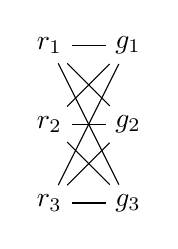
\begin{tikzpicture}
  \graph [color class=red, color class=green, math nodes]
  { [complete bipartite={red}{green}]
    { [red,   Cartesian placement]                      r_1, r_2, r_3 },
    { [green, Cartesian placement, nodes={xshift=1cm}]  g_1, g_2, g_3 }
  };
\end{tikzpicture}
\end{codeexample}

A list of predefined joining operators can be found in the reference
Section~\ref{section-library-graphs-reference}.

The fact that joining operators can also be used as normal operators leads to a
subtle problem: A normal operator will typically use the current value of
|default edge kind| to decide which kind of edges should be put between the
identified vertices, while a joining operator should, naturally, use the kind
of edge specified by the \meta{edge specification}. This problem is solved as
follows: Like a normal operator, a joining operator should also use the current
value of |default edge kind| for the edges it produces. The trick is that this
will automatically be set to the current \meta{edge specification} when the
operator explicitly in the \meta{options} of the edge specification or
implicitly in the |default edge operator|.


\subsection{Graph Macros}
\label{section-library-graphs-macros}

A \emph{graph macro} is a small graph that is inserted at some point into the
graph that is currently being constructed. There is special support for such
graph macros in \tikzname. You might wonder why this is necessary -- can't one
use \TeX's normal macro mechanism? The answer is ``no'': one cannot insert new
nodes into a graph using normal macros because the chains, groups, and nodes
are determined prior to macro expansion. Thus, any macro encountered where some
node text should go will only be expanded when this node is being named and
typeset.

A graph macro is declared using the following key:

\begin{key}{/tikz/graphs/declare=\marg{graph name}\marg{specification}}
    This key declares that \meta{graph name} can subsequently be used as a
    replacement for a \meta{node name}. Whenever the \meta{graph name} is used
    in the following, a graph group will be inserted instead whose content is
    exactly \meta{specification}. In case \meta{graph name} is used together
    with some \meta{options}, they are executed prior to inserting the
    \meta{specification}.
    %
\begin{codeexample}[]
\tikz \graph [branch down=4mm, declare={claw}{1 -- {2,3,4}}] {
  a;
  claw;
  b;
};
\end{codeexample}
    %
    In the next example, we use a key to configure a subgraph:
    %
\begin{codeexample}[]
\tikz \graph [ n/.code=\def\n{#1}, branch down=4mm,
               declare={star}{root -- { \foreach \i in {1,...,\n} {\i} }}]
{ star [n=5]; };
\end{codeexample}
    %
    Actually, the |n| key is already defined internally for a similar purpose.

    As a last example, let us define a somewhat more complicated graph macro.
    %
\begin{codeexample}[]
\newcount\mycount
\tikzgraphsset{
  levels/.store in=\tikzgraphlevel,
  levels=1,
  declare={bintree}{%
    [/utils/exec={%
      \ifnum\tikzgraphlevel=1\relax%
        \def\childtrees{ / }%
      \else%
        \mycount=\tikzgraphlevel%
        \advance\mycount by-1\relax%
        \edef\childtrees{
          / -> {
            bintree[levels=\the\mycount],
            bintree[levels=\the\mycount]
          }}
      \fi%
    },
    parse/.expand once=\childtrees
    ]
    % Everything is inside the \childtrees...
  }
}
\tikz \graph [grow down=5mm, branch right=5mm] { bintree [levels=5] };
\end{codeexample}
    %
\end{key}

Note that when you use a graph macro several time inside the same graph, you
will typically have to use the |name| option so that different copies of the
subgraph are created:
%
\begin{codeexample}[]
\tikz \graph [branch down=4mm, declare={claw}{1 -- {2,3,4}}] {
  claw [name=left],
  claw [name=right]
};
\end{codeexample}

You will find a list of useful graph macros in the reference section,
Section~\ref{section-library-graphs-reference-macros}.


\subsection{Online Placement Strategies}
\label{section-library-graphs-placement}

The main job of the |graphs| library is to make it easy to specify which nodes
are present in a graph and how they are connected. In contrast, it is
\emph{not} the primary job of the library to compute good positions for nodes
in a graph -- use for instance a |\matrix|, specify good positions ``by hand''
or use the graph drawing facilities. Nevertheless, some basic support for
automatic node placement is provided for simple cases. The graph library will
provide you with information about the position of nodes inside their groups
and chains.

As a graph is being constructed, a \emph{placement strategy} is used to
determine a (reasonably good) position for the nodes as they are created. These
placement strategies get some information about what \tikzname\ has already
seen concerning the already constructed nodes, but it gets no information
concerning the upcoming nodes. Because of this lack of information concerning
the future, the strategies need to be what is called an \emph{online strategy}
in computer science. (The opposite are \emph{offline strategies}, which get
information about the whole graph and all the sizes of the nodes in it. The
graph drawing libraries employ such offline strategies.)

Strategies are selected using keys like |no placement| or
|Cartesian placement|. It is permissible to use different strategies inside
different parts of a graph, even though the different strategies do not always
work together in perfect harmony.


\subsubsection{Manual Placement}
\label{section-graphs-xy}

\begin{key}{/tikz/graphs/no placement}
    This strategy simply ``switches off'' the whole placement mechanism,
    causing all nodes to be placed at the origin by default. You need to use
    this strategy if you position nodes ``by hand''. For this, you can use the
    |at| key, the |shift| keys:
    %
\begin{codeexample}[]
\tikz \graph [no placement]
{
  a[at={(0:0)}] -> b[at={(1,0)}] -> c[yshift=1cm];
};
\end{codeexample}
    %
    Since the syntax and the many braces and parentheses are a bit cumbersome,
    the following two keys might also be useful:
    %
    \begin{key}{/tikz/graphs/x=\meta{x dimension}}
        When you use this key, it will have the same effect as if you had
        written |at={(|\meta{x dimension}|,|\meta{y dimension}|)}|, where
        \meta{y dimension} is a value set using the |y| key:
        %
\begin{codeexample}[]
\tikz \graph [no placement]
{
  a[x=0,y=0] -> b[x=1,y=0] -> c[x=0,y=1];
};
\end{codeexample}
        %
        Note that you can specify an |x| or a |y| key for a whole scope and
        then vary only the other key:
        %
\begin{codeexample}[]
\tikz \graph [no placement]
{
  a ->
  { [x=1] % group option
    b [y=0] -> c[y=1]
  };
};
\end{codeexample}
        %
        Note that these keys have the path |/tikz/graphs/|, so they will be
        available inside |graph|s and will not clash with the usual |x| and |y|
        keys of \tikzname, which are used to specify the basic lengths of
        vectors.
    \end{key}
    %
    \begin{key}{/tikz/graphs/y=\meta{y dimension}}
        See above.
    \end{key}
\end{key}


\subsubsection{Placement on a Grid}

\begin{key}{/tikz/graphs/Cartesian placement}
    This strategy is the default strategy. It works, roughly, as follows: For
    each new node on a chain, advance a ``logical width'' counter and for each
    new node in a group, advance a ``logical depth'' counter. When a chain
    contains a whole group, then the ``logical width'' taken up by the group is
    the maximum over the logical widths taken up by the chains inside the
    group; and symmetrically the logical depth of a chain is the maximum of the
    depths of the groups inside it.

    This slightly confusing explanation is perhaps best exemplified. In the
    below example, the two numbers indicate the two logical width and depth of
    each node as computed by the |graphs| library. Just ignore the arcane code
    that is used to print these numbers.
    %
\begin{codeexample}[]
\tikz
  \graph [nodes={align=center, inner sep=1pt}, grow right=7mm,
          typeset={\tikzgraphnodetext\\[-4pt]
                   \tiny\mywidth\\[-6pt]\tiny\mydepth},
          placement/compute position/.append code=
            \pgfkeysgetvalue{/tikz/graphs/placement/width}{\mywidth}
            \pgfkeysgetvalue{/tikz/graphs/placement/depth}{\mydepth}]
{
  a,
  b,
  c -> d -> {
    e -> f -> g,
    h -> i
  } -> j,
  k -> l
};
\end{codeexample}
    %
    You will find a detailed description of how these logical units are
    computed, exactly, in Section~\ref{section-library-graphs-new-online}.

    Now, even though we talk about ``widths'' and ``depths'' and even though by
    default a graph ``grows'' to the right and down, this is by no means fixed.
    Instead, you can use the following keys to change how widths and heights
    are interpreted:
    %
    \begin{key}{/tikz/graphs/chain shift=\meta{coordinate} (initially {(1,0)})}
        Under the regime of the |Cartesian placement| strategy, each node is
        shifted by the current logical width times this \meta{coordinate}.
        %
\begin{codeexample}[]
\tikz \graph [chain shift=(45:1)] {
  a -> b -> c;
  d -> e;
  f -> g -> h;
};
\end{codeexample}
    \end{key}
    %
    \begin{key}{/tikz/graphs/group shift=\meta{coordinate} (initially {(0,-1)})}
        Like for |chain shift|, each node is shifted by the current logical
        depth times this \meta{coordinate}.
        %
\begin{codeexample}[]
\tikz \graph [chain shift=(45:7mm), group shift=(-45:7mm)] {
  a -> b -> c;
  d -> e;
  f -> g -> h;
};
\end{codeexample}
    \end{key}
\end{key}

\begin{key}{/tikz/graphs/grow up=\meta{distance} (default 1)}
    Sets the |chain shift| to |(|\meta{distance}|,0)|, so that chains ``grow
    upward''. The distance by which the center of each new element is removed
    from the center of the previous one is \meta{distance}.
    %
\begin{codeexample}[]
\tikz \graph [grow up=7mm] { a -> b -> c};
\end{codeexample}
    %
\end{key}

\begin{key}{/tikz/graphs/grow down=\meta{distance} (default 1)}
    Like |grow up|.
    %
\begin{codeexample}[]
\tikz \graph [grow down=7mm] { a -> b -> c};
\end{codeexample}
    %
\end{key}

\begin{key}{/tikz/graphs/grow left=\meta{distance} (default 1)}
    Like |grow up|.
    %
\begin{codeexample}[]
\tikz \graph [grow left=7mm] { a -> b -> c};
\end{codeexample}
    %
\end{key}

\begin{key}{/tikz/graphs/grow right=\meta{distance} (default 1)}
    Like |grow up|.
    %
\begin{codeexample}[]
\tikz \graph [grow right=7mm] { a -> b -> c};
\end{codeexample}
    %
\end{key}

\begin{key}{/tikz/graphs/branch up=\meta{distance} (default 1)}
    Sets the |group shift| so that groups ``branch upward''.  The distance by
    which the center of each new element is removed from the center of the
    previous one is \meta{distance}.
    %
\begin{codeexample}[]
\tikz \graph [branch up=7mm] { a -> b -> {c, d, e} };
\end{codeexample}
    %
    Note that when you draw a tree, the |branch ...| keys specify how siblings
    (or adjacent branches) are arranged, while the |grow ...| keys specify in
    which direction the branches ``grow''.
\end{key}

\begin{key}{/tikz/graphs/branch down=\meta{distance} (default 1)}
%
\begin{codeexample}[]
\tikz \graph [branch down=7mm] { a -> b -> {c, d, e}};
\end{codeexample}
%
\end{key}

\begin{key}{/tikz/graphs/branch left=\meta{distance} (default 1)}
%
\begin{codeexample}[]
\tikz \graph [branch left=7mm, grow down=7mm] { a -> b -> {c, d, e}};
\end{codeexample}
%
\end{key}

\begin{key}{/tikz/graphs/branch right=\meta{distance} (default 1)}
%
\begin{codeexample}[]
\tikz \graph [branch right=7mm, grow down=7mm] { a -> b -> {c, d, e}};
\end{codeexample}
%
\end{key}

The following keys place nodes in a $N\times M$ grid.
%
\begin{key}{/tikz/graphs/grid placement}
    This key works similar to |Cartesian placement|. As for that placement
    strategy, a node has logical width and depth 1. However, the computed total
    width and depth are mapped to a $N\times M$ grid. The values of $N$ and $M$
    depend on the size of the graph and the value of |wrap after|. The number
    of columns $M$ is either set to |wrap after| explicitly or computed
    automatically as $\sqrt{\texttt{\string|V\string|}}$. $N$ is the number of
    rows needed to lay out the graph in a grid with $M$ columns.
    %
\begin{codeexample}[preamble={\usetikzlibrary{graphs.standard}}]
% An example with 6 nodes, 3 columns and therefor 2 rows
\tikz \graph [grid placement] { subgraph I_n[n=6, wrap after=3] };
\end{codeexample}
    %
\begin{codeexample}[preamble={\usetikzlibrary{graphs.standard}}]
% An example with 9 nodes with columns and rows computed automatically
\tikz \graph [grid placement] { subgraph Grid_n [n=9] };
\end{codeexample}
    %
\begin{codeexample}[preamble={\usetikzlibrary{graphs.standard}}]
% Directions can be changed
\tikz \graph [grid placement, branch up, grow left] { subgraph Grid_n [n=9] };
\end{codeexample}
    %
    In case a user-defined graph instead of a pre-defined |subgraph| is to be
    laid out using |grid placement|, |n| has to be specified explicitly:
    %
\begin{codeexample}[]
\tikz \graph [grid placement] {
  [n=6, wrap after=3]
  a -- b -- c -- d -- e -- f
};
\end{codeexample}
    %
\end{key}


\subsubsection{Placement Taking Node Sizes Into Account}

Options like |grow up| or |branch right| do not take the sizes of the
to-be-positioned nodes into account -- all nodes are placed quite ``dumbly'' at
grid positions. It turns out that the |Cartesian placement| can also be used to
place notes in such a way that their height and/or width is taken into account.
Note, however, that while the following options may yield an adequate placement
in many situations, when you need advanced alignments you should use a |matrix|
or advanced offline strategies to place the nodes.

\begin{key}{/tikz/graphs/grow right sep=\meta{distance} (default 1em)}
    This key has several effects, but let us start with the bottom line: Nodes
    along a chain are placed in such a way that the left end of a new node is
    \meta{distance} from the right end of the previous node:
    %
\begin{codeexample}[]
\tikz \graph [grow right sep, left anchor=east, right anchor=west] {
  start -- {
    long text -- {short, very long text} -- more text,
    long -- longer -- longest
  } -- end
};
\end{codeexample}
    %
    What happens internally is the following: First, the |anchor| of the nodes
    is set to |west| (or |north west| or |south west|, see below). Second, the
    logical width of a node is no longer |1|, but set to the actual width of
    the node (which we define as the horizontal difference between the |west|
    anchor and the |east| anchor) in points. Third, the |chain shift| is set to
    |(1pt,0pt)|.
\end{key}

\begin{key}{/tikz/graphs/grow left sep=\meta{distance} (default 1em)}
%
\begin{codeexample}[]
\tikz \graph [grow left sep] { long -- longer -- longest };
\end{codeexample}
%
\end{key}

\begin{key}{/tikz/graphs/grow up sep=\meta{distance} (default 1em)}
\begin{codeexample}[]
\tikz \graph [grow up sep] {
  a / $a=x$ --
  b / {$b=\displaystyle \int_0^1 x dx$} --
  c [draw, circle, inner sep=7mm]
};
\end{codeexample}
%
\end{key}

\begin{key}{/tikz/graphs/grow down sep=\meta{distance} (default 1em)}
    As above.
\end{key}

\begin{key}{/tikz/graphs/branch right sep=\meta{distance} (default 1em)}
    This key works like |grow right sep|, only it affects groups rather than
    chains.
    %
\begin{codeexample}[]
\tikz \graph [grow down, branch right sep] {
  start -- {
    an even longer text -- {short, very long text} -- more text,
    long -- longer -- longest,
    some text -- a -- b
  } -- end
};
\end{codeexample}
    %
    When both this key and, say, |grow down sep| are set, instead of the |west|
    anchor, the |north west| anchor will be selected automatically.
\end{key}

\begin{key}{/tikz/graphs/branch left sep=\meta{distance} (default 1em)}
%
\begin{codeexample}[]
\tikz \graph [grow down sep, branch left sep] {
  start -- {
    an even longer text -- {short, very long text} -- more text,
    long -- longer,
    some text -- a -- b
  } -- end
};
\end{codeexample}
%
\end{key}

\begin{key}{/tikz/graphs/branch up sep=\meta{distance} (default 1em)}
%
\begin{codeexample}[]
\tikz \graph [branch up sep] { a, b, c[draw, circle, inner sep=7mm] };
\end{codeexample}
%
\end{key}

\begin{key}{/tikz/graphs/branch down sep=\meta{distance} (default 1em)}
\end{key}


\subsubsection{Placement On a Circle}

The following keys place nodes on circles. Note that, typically, you do not use
|circular placement| directly, but rather use one of the two keys |clockwise|
or |counterclockwise|.

\begin{key}{/tikz/graphs/circular placement}
    This key works quite similar to |Cartesian placement|. As for that
    placement strategy, a node has logical width and depth |1|. However, the
    computed total width and depth are mapped to polar coordinates rather than
    Cartesian coordinates.

    \begin{key}{/tikz/graphs/chain polar shift=|(|\meta{angle}|:|\meta{radius}|)| (initially {(0:1)})}
        Under the regime of the |circular placement| strategy, each node on a
        chain is shifted by
        |(|\meta{logical width}\meta{angle}|:|\meta{logical width}\meta{angle}|)|.
        %
\begin{codeexample}[]
\tikz \graph [circular placement] {
  a -> b -> c;
  d -> e;
  f ->  g -> h;
};
\end{codeexample}
        %
    \end{key}
    %
    \begin{key}{/tikz/graphs/group polar shift=|(|\meta{angle}|:|\meta{radius}|)| (initially {(45:0)})}
        Like for |group shift|, each node on a chain is shifted by
        |(|\meta{logical depth}\meta{angle}|:|\meta{logical depth}\meta{angle}|)|.
        %
\begin{codeexample}[]
\tikz \graph [circular placement, group polar shift=(30:0)] {
  a -> b -> c;
  d -> e;
  f -> g -> h;
};
\end{codeexample}
        %
\begin{codeexample}[]
\tikz \graph [circular placement,
              chain polar shift=(30:0),
              group polar shift=(0:1cm)] {
  a -- b -- c;
  d -- e;
  f -- g -- h;
};
\end{codeexample}
    \end{key}
    %
    \begin{key}{/tikz/graphs/radius=\meta{dimension} (initially 1cm)}
        This is an initial value that is added to the total computed radius
        when the polar shift of a node has been calculated. Essentially, this
        key allows you to set the \meta{radius} of the innermost circle.
        %
\begin{codeexample}[]
\tikz \graph [circular placement, radius=5mm] { a, b, c, d };
\end{codeexample}
        %
\begin{codeexample}[]
\tikz \graph [circular placement, radius=1cm] { a, b, c, d };
\end{codeexample}
    \end{key}
    %
    \begin{key}{/tikz/graphs/phase=\meta{angle} (initially 90)}
        This is an initial value that is added to the total computed angle when
        the polar shift of a node has been calculated.
        %
\begin{codeexample}[]
\tikz \graph [circular placement] { a, b, c, d };
\end{codeexample}
        %
\begin{codeexample}[]
\tikz \graph [circular placement, phase=0] { a, b, c, d };
\end{codeexample}
    \end{key}
\end{key}

\label{key-graphs-clockwise}%
\begin{key}{/tikz/graphs/clockwise=\meta{number} (default \string\tikzgraphVnum)}
    This key sets the |group shift| so that if there are exactly \meta{number}
    many nodes in a group, they will form a complete circle. If you do not
    provide a \meta{number}, the current value of |\tikzgraphVnum| is used,
    which is exactly what you want when you use predefined graph macros like
    |subgraph K_n|.
    %
\begin{codeexample}[]
\tikz \graph [clockwise=4] { a, b, c, d };
\end{codeexample}
    %
\begin{codeexample}[preamble={\usetikzlibrary{graphs.standard}}]
\tikz \graph [clockwise] { subgraph K_n [n=5] };
\end{codeexample}
    %
\end{key}

\label{key-graphs-counterclockwise}%
\begin{key}{/tikz/graphs/counterclockwise=\meta{number} (default \string\tikzgraphVnum)}
    Works like |clockwise|, only the direction is inverted.
\end{key}


\subsubsection{Levels and Level Styles}

As a graph is being parsed, the |graph| command keeps track of a parameter
called the \emph{level} of a node. Provided that the graph is actually
constructed in a tree-like manner, the level is exactly equal to the level of
the node inside this tree.

\begin{key}{/tikz/graphs/placement/level}
    This key stores a number that is increased for each element on a chain, but
    gets reset at the end of a group:
    %
\begin{codeexample}[]
\tikz \graph [ branch down=5mm, typeset=
    \tikzgraphnodetext:\pgfkeysvalueof{/tikz/graphs/placement/level}]
{
  a -> {
    b,
    c -> {
      d,
      e -> {f,g},
      h
    },
    j
  }
};
\end{codeexample}
    %
    Unlike the parameters |depth| and |width| described in the next section,
    the key |level| is always available.
\end{key}

In addition to keeping track of the value of the |level| key, the |graph|
command also executes the following keys whenever it creates a node:

\begin{stylekey}{/tikz/graph/level=\meta{level}}
    This key gets executed for each newly created node with \meta{level} set to
    the current level of the node. You can use this key to, say, reconfigure
    the node distance or the node color.
\end{stylekey}

\begin{stylekey}{/tikz/graph/level \meta{level}}
    This key also gets executed for each newly created node with \meta{level}
    set to the current level of the node.
    %
\begin{codeexample}[]
\tikz \graph [
  branch down=5mm,
  level 1/.style={nodes=red},
  level 2/.style={nodes=green!50!black},
  level 3/.style={nodes=blue}]
{
  a -> {
    b,
    c -> {
      d,
      e -> {f,g},
      h
    },
    j
  }
};
\end{codeexample}
    %
\begin{codeexample}[]
\tikz \graph [
  branch down=5mm,
  level 1/.style={grow right=2cm},
  level 2/.style={grow right=1cm},
  level 3/.style={grow right=5mm}]
{
  a -> {
    b,
    c -> {
      d,
      e -> {f,g},
      h
    },
    j
  }
};
\end{codeexample}
    %
\end{stylekey}


\subsubsection{Defining New Online Placement Strategies}
\label{section-library-graphs-new-online}

In the following the details of how to define a new placement strategy are
explained. Most readers may wish to skip this section.

As a graph specification is being parsed, the |graphs| library will keep track
of different numbers that identify the positions of the nodes. Let us start
with what happens on a chain. First, the following counter is increased for
each element of the chain:
%
\begin{key}{/tikz/graphs/placement/element count}
    This key stores a number that tells us the position of the node on the
    current chain. However, you only have access to this value inside the code
    passed to the macro |compute position|, explained later on.
    %
\begin{codeexample}[]
\tikz \graph [
  grow right sep, typeset=\tikzgraphnodetext:\mynum,
  placement/compute position/.append code=
    \pgfkeysgetvalue{/tikz/graphs/placement/element count}{\mynum}]
{
  a -> b -> c,
  d -> {e, f->h} -> j
};
\end{codeexample}
    %
    As can be seen, each group resets the element counter.
\end{key}

The second value that is computed is more complicated to explain, but it also
gives more interesting information:
%
\begin{key}{/tikz/graphs/placement/width}
    This key stores the ``logical width'' of the nodes parsed up to now in the
    current group or chain (more precisely, parsed since the last call of
    |place| in an enclosing group). This is not necessarily the ``total
    physical width'' of the nodes, but rather a number representing how ``big''
    the elements prior to the current element were. This \emph{may} be their
    width, but it may also be their height or even their number (which,
    incidentally, is the default). You can use the |width| to perform shifts or
    rotations of to-be-created nodes (to be explained later).

    The logical width is defined recursively as follows. First, the width of a
    single node is computed by calling the following key:
    %
    \begin{key}{/tikz/graphs/placement/logical node width=\meta{full node name}}
        This key is called to compute a physical or logical width of the node
        \meta{full node name}. You can change the code of this key. The code
        should return the computed value in the macro |\pgfmathresult|. By
        default, this key returns |1|.
    \end{key}
    %
    The width of a chain is the sum of the widths of its elements. The width of
    a group is the maximum of the widths of its elements.

    To get a feeling what the above rules imply in practice, let us first have
    a look at an example where each node has logical width and height |1|
    (which is the default). The arcane options at the beginning of the code
    just setup things so that the computed width and depth of each node is
    displayed at the bottom of each node.
    %
\begin{codeexample}[]
\tikz
  \graph [nodes={align=center, inner sep=1pt}, grow right=7mm,
          typeset={\tikzgraphnodetext\\[-4pt]
                   \tiny\mywidth\\[-6pt]\tiny\mydepth},
          placement/compute position/.append code=
            \pgfkeysgetvalue{/tikz/graphs/placement/width}{\mywidth}
            \pgfkeysgetvalue{/tikz/graphs/placement/depth}{\mydepth}]
{
  a,
  b,
  c -> d -> {
    e -> f -> g,
    h -> i
  } -> j,
  k -> l
};
\end{codeexample}
    %
    In the next example the ``logical'' width and depth actually match the
    ``physical'' width and height. This is caused by the |grow right sep|
    option, which internally sets the |logical node width| key so that it
    returns the width of its parameter in points.
    %
\begin{codeexample}[]
\tikz
  \graph [grow right sep, branch down sep, nodes={align=left, inner sep=1pt},
          typeset={\tikzgraphnodetext\\[-4pt] \tiny Width: \mywidth\\[-6pt] \tiny Depth: \mydepth},
          placement/compute position/.append code=
            \pgfkeysgetvalue{/tikz/graphs/placement/width}{\mywidth}
            \pgfkeysgetvalue{/tikz/graphs/placement/depth}{\mydepth}]
{
  a,
  b,
  c -> d -> {
    e -> f -> g,
    h -> i
  } -> j,
  k -> l
};
\end{codeexample}
    %
\end{key}

Symmetrically to chains, as a group is being constructed, counters are
available for the number of chains encountered so far in the current group and
for the logical depth of the current group:
%
\begin{key}{/tikz/graphs/placement/element count}
    This key stores a number that tells us the sequence number of the
    chain in the current group.
    %
\begin{codeexample}[]
\tikz \graph [
  grow right sep, branch down=5mm, typeset=\tikzgraphnodetext:\mynum,
  placement/compute position/.append code=
    \pgfkeysgetvalue{/tikz/graphs/placement/chain count}{\mynum}]
{
  a -> b -> {c,d,e},
  f,
  g -> h
};
\end{codeexample}
    %
\end{key}

\begin{key}{/tikz/graphs/placement/depth}
    Similarly to the |width| key, this key stores the ``logical depth'' of the
    nodes parsed up to now in the current group or chain and, also similarly,
    this key may or may not be related to the actual depth/height of the
    current node. As for the |width|, the exact definition is as follows: For a
    single node, the depth is computed by the following key:
    %
    \begin{key}{/tikz/graphs/placement/logical node depth=\meta{full node name}}
        The code behind this key should return the ``logical height'' of the
        node \meta{full node name} in the macro |\pgfmathresult|.
    \end{key}
    %
    Second, the depth of a group is the sum of the depths of its elements.
    Third, the depth of a chain is the maximum of the depth of its elements.
\end{key}

The |width|, |depth|, |element count|, and |chain count| keys get updated
automatically, but do not have an effect by themselves. This is to the
following two keys:

\begin{key}{/tikz/graphs/placement/compute position=\meta{code}}
    The \meta{code} is called by the |graph| command just prior to creating a
    new node (the exact moment when this key is called is detailed in the
    description of the |place| key). When the \meta{code} is called, all of the
    keys described above will hold numbers computed in the way described above.

    The job of the \meta{code} is to setup node options appropriately so that
    the to-be-created node will be placed correctly. Thus, the \meta{code}
    should typically set the key |nodes={shift=|\meta{coordinate}|}| where
    \meta{coordinate} is the computed position for the node. The \meta{code}
    could also set other options like, say, the color of a node depending on
    its depth.

    The following example appends some code to the standard code of
    |compute position| so that ``deeper'' nodes of a tree are lighter.
    (Naturally, the same effect could be achieved much more easily using the
    |level| key.)
    %
\begin{codeexample}[]
\newcount\mycount
\def\lightendeepernodes{
  \pgfmathsetcount{\mycount}{
    100-20*\pgfkeysvalueof{/tikz/graphs/placement/width}
  }
  \edef\mydepth{\the\mycount}
  \tikzset{nodes={fill=red!\mydepth,circle,text=white}}
}
\tikz
  \graph [placement/compute position/.append code=\lightendeepernodes]
   {
     a -> {
       b -> c -> d,
       e -> {
         f,
         g
       },
       h
     }
   };
\end{codeexample}
    %
\end{key}

\begin{key}{/tikz/graphs/placement/place}
    Executing this key has two effects: First, the key |compute position| is
    called to compute a good position for future nodes (usually, these ``future
    nodes'' are just a single node that is created immediately). Second, all of
    the above counters like |depth| or |width| are reset (but not |level|).

    There are two places where this key is sensibly called: First, just prior
    to creating a node, which happens automatically. Second, when you change
    the online strategy. In this case, the computed width and depth values from
    one strategy typically make no sense in the other strategy, which is why
    the new strategy should proceed ``from a fresh start''. In this case, the
    implicit call of |compute position| ensures that the new strategy gets the
    last place the old strategy would have used as its starting point, while
    the computation of its positions is now relative to this new starting
    point.

    For these reasons, when an online strategy like |Cartesian placement| is
    called, this key gets called implicitly. You will rarely need to call this
    key directly, except when you define a new online strategy.
\end{key}


\subsection{Reference: Predefined Elements}
\label{section-library-graphs-reference}

\subsubsection{Graph Macros}
\label{section-library-graphs-reference-macros}

\begin{tikzlibrary}{graphs.standard}
    This library defines a number of graph macros that are often used in the
    literature. When new graphs are added to this collection, they will follow
    the definitions in the Mathematica program, see
    \url{mathworld.wolfram.com/topics/SimpleGraphs.html}.
\end{tikzlibrary}

\begin{graph}{subgraph I\_n}
    This graph consists just of $n$ unconnected vertices. The following key is
    used to specify the set of these vertices:
    %
    \begin{key}{/tikz/graphs/V=\marg{list of vertices}}
        Sets a list of vertex names for use with graphs like |subgraph I_n| and
        also other graphs. This list is available in the macro |\tikzgraphV|.
        The number of elements of this list is available in |\tikzgraphVnum|.
    \end{key}
    %
    \begin{key}{/tikz/graphs/n=\meta{number}}
        This is an abbreviation for
        |V={1,...,|\meta{number}|}, name shore V/.style={name=V}|.
    \end{key}
    %
\begin{codeexample}[preamble={\usetikzlibrary{graphs.standard}}]
\tikz \graph [branch right, nodes={draw, circle}]
  { subgraph I_n [V={a,b,c}] };
\end{codeexample}
    %
    This graph is not particularly exciting by itself. However, it is often
    used to introduce nodes into a graph that are then connected as in the
    following example:
    %
\begin{codeexample}[preamble={\usetikzlibrary{graphs.standard}}]
\tikz \graph [clockwise, clique] { subgraph I_n [n=4] };
\end{codeexample}
    %
\end{graph}

\begin{graph}{subgraph I\_nm}
    This graph consists of two sets of once $n$ unconnected vertices and then
    $m$ unconnected vertices. The first set consists of the vertices set by the
    key |V|, the other set consists of the vertices set by the key |W|.
    %
\begin{codeexample}[preamble={\usetikzlibrary{graphs.standard}}]
\tikz \graph { subgraph I_nm [V={1,2,3}, W={a,b,c}] };
\end{codeexample}
    %
    In order to set the graph path name of the two sets, the following keys get
    executed:
    %
    \begin{stylekey}{/tikz/graphs/name shore V (initially \normalfont empty)}
        Set this style to, say, |name=my V set| in order to set a name for the
        |V| set.
    \end{stylekey}
    %
    \begin{stylekey}{/tikz/graphs/name shore W (initially \normalfont empty)}
        Same as for |name shore V|.
    \end{stylekey}
    %
    \begin{key}{/tikz/graphs/W=\marg{list of vertices}}
        Sets the list of vertices for the |W| set. The elements and their
        number are available in the macros |\tikzgraphW| and |\tikzgraphWnum|,
        respectively.
    \end{key}
    %
    \begin{key}{/tikz/graphs/m=\meta{number}}
        This is an abbreviation for
        |W={1,...,|\meta{number}|}, name shore W/.style={name=W}|.
    \end{key}
    %
    The main purpose of this subgraph is to setup the nodes in a bipartite
    graph:
    %
\begin{codeexample}[preamble={\usetikzlibrary{graphs.standard}}]
\tikz \graph {
  subgraph I_nm [n=3, m=4];

  V 1 -- { W 2, W 3 };
  V 2 -- { W 1, W 3 };
  V 3 -- { W 1, W 4 };
};
\end{codeexample}
    %
\end{graph}

\begin{graph}{subgraph K\_n}
    This graph is the complete clique on the vertices from the |V| key.
    %
\begin{codeexample}[preamble={\usetikzlibrary{graphs.standard}}]
\tikz \graph [clockwise] { subgraph K_n [n=7] };
\end{codeexample}
    %
\end{graph}

\begin{graph}{subgraph K\_nm}
    This graph is the complete bipartite graph with the two shores |V| and |W|
    as in |subgraph I_nm|.
    %
\begin{codeexample}[preamble={\usetikzlibrary{graphs.standard}}]
\tikz \graph [branch right, grow down]
  { subgraph K_nm [V={6,...,9}, W={b,...,e}] };
\end{codeexample}
    %
\begin{codeexample}[preamble={\usetikzlibrary{graphs.standard}}]
\tikz \graph [simple, branch right, grow down]
{
  subgraph K_nm [V={1,2,3}, W={a,b,c,d}, ->];
  subgraph K_nm [V={2,3},   W={b,c},     <-];
};
\end{codeexample}
    %
\end{graph}

\begin{graph}{subgraph P\_n}
    This graph is the path on the vertices in |V|.
    %
\begin{codeexample}[preamble={\usetikzlibrary{graphs.standard}}]
\tikz \graph [branch right] { subgraph P_n [n=3] };
\end{codeexample}
    %
\end{graph}

\begin{graph}{subgraph C\_n}
    This graph is the cycle on the vertices in |V|.
    %
\begin{codeexample}[preamble={\usetikzlibrary{graphs.standard}}]
\tikz \graph [clockwise] { subgraph C_n [n=7, ->] };
\end{codeexample}
    %
\end{graph}

\begin{graph}{subgraph Grid\_n}
    This graph is a grid of the vertices in |V|.
    %
    \begin{key}{/tikz/graphs/wrap after=\meta{number}}
        Defines the number of nodes placed in a single row of the grid. This
        value implicitly defines the number of grid columns as well. In the
        following example a |grid placement| is used to visualize the edges
        created between the nodes of a |Grid_n| |subgraph| using different
        values for |wrap after|.
        %
\begin{codeexample}[preamble={\usetikzlibrary{graphs.standard}}]
\tikz \graph [grid placement] { subgraph Grid_n [n=3,wrap after=1] };
\tikz \graph [grid placement] { subgraph Grid_n [n=3,wrap after=3] };
\end{codeexample}
        %
\begin{codeexample}[preamble={\usetikzlibrary{graphs.standard}}]
\tikz \graph [grid placement] { subgraph Grid_n [n=4,wrap after=2] };
\tikz \graph [grid placement] { subgraph Grid_n [n=4] };
\end{codeexample}
  \end{key}
\end{graph}

% TODO: Implement the Grid_nm subgraph described here:
%
%\begin{graph}{subgraph Grid\_nm}
%  This graph is a grid built from the cartesian product of the two node
%  sets |V| and |W| which are either defined using the keys
%  |/tikz/graphs/V| and |/tikz/graphs/W| or |/tikz/graphs/n| and
%  |/tikz/graphs/m| or a mixture of both.
%
%  The resulting |Grid_nm| subgraph has $n$ ``rows'' and $m$ ``columns'' and
%  the nodes are named |V i W j| with $1\le i\le n$ and $1\le j\le n$.
%  The names of the two shores |V| and |W| can be changed as described in
%  the documentation of the keys |/tikz/graphs/name shore V| and
%  |/tikz/graphs/name shore W|.
%  \begin{codeexample}[]
%\tikz \graph [grid placement] { subgraph Grid_nm [V={1,2,3}, W={4, 5, 6}] };
%  \end{codeexample}
%\end{graph}


\subsubsection{Group Operators}

The following keys use the |operator| key to setup operators that connect the
vertices of the current group having a certain color in a specific way.

\begin{key}{/tikz/graphs/clique=\meta{color} (default all)}
    Adds an edge between all vertices of the current group having the (logical)
    color \meta{color}. Since, by default, this color is set to |all|, which is
    a color that all nodes get by default, when you do not specify anything,
    all nodes will be connected.
    %
\begin{codeexample}[]
\tikz \graph [clockwise, n=5] {
  a,
  b,
  {
    [clique]
    c, d, e
  }
};
\end{codeexample}
    %
\begin{codeexample}[]
\tikz \graph [color class=red, clockwise, n=5] {
  [clique=red, ->]
  a, b[red], c[red], d, e[red]
};
\end{codeexample}
    %
\end{key}

\begin{key}{/tikz/graphs/induced independent set=\meta{color} (default all)}
    This key is the ``opposite'' of a |clique|: It removes all edges in the
    current group having belonging to color class \meta{color}. More precisely,
    an edge of kind |-!-| is added for each pair of vertices. This means that
    edge only get removed if you specify the |simple| option.
    %
\begin{codeexample}[preamble={\usetikzlibrary{graphs.standard}}]
\tikz \graph [simple] {
  subgraph K_n [<->, n=7, clockwise]; % create lots of edges

  { [induced independent set] 1, 3, 4, 5, 6 }
};
\end{codeexample}
    %
\end{key}

\begin{key}{/tikz/graphs/cycle=\meta{color} (default all)}
    Connects the nodes colored \meta{color} is a cyclic fashion. The ordering
    is the ordering in which they appear in the whole graph specification.
    %
\begin{codeexample}[]
\tikz \graph [clockwise, n=6, phase=60] {
  { [cycle, ->] a, b, c },
  { [cycle, <-] d, e, f }
};
\end{codeexample}
    %
\end{key}

\begin{key}{/tikz/graphs/induced cycle=\meta{color} (default all)}
    While the |cycle| command will only add edges, this key will also remove
    all other edges between the nodes of the cycle, provided we are
    constructing a |simple| graph.
    %
\begin{codeexample}[preamble={\usetikzlibrary{graphs.standard}}]
\tikz \graph [simple] {
  subgraph K_n [n=7, clockwise]; % create lots of edges

  { [induced cycle, ->, edge=red] 2, 3, 4, 6, 7 },
};
\end{codeexample}
    %
\end{key}

\begin{key}{/tikz/graphs/path=\meta{color} (default all)}
    Works like |cycle|, only there is no edge from the last to the first
    vertex.
    %
\begin{codeexample}[]
\tikz \graph [clockwise, n=6] {
  { [path, ->] a, b, c },
  { [path, <-] d, e, f }
};
\end{codeexample}
    %
\end{key}

\begin{key}{/tikz/graphs/induced path=\meta{color} (default all)}
    Works like |induced cycle|, only there is no edge from the last to the
    first vertex.
    %
\begin{codeexample}[preamble={\usetikzlibrary{graphs.standard}}]
\tikz \graph [simple] {
  subgraph K_n [n=7, clockwise]; % create lots of edges

  { [induced path, ->, edges=red] 2, 3, 4, 6, 7 },
};
\end{codeexample}
    %
\end{key}


\subsubsection{Joining Operators}

The following keys are typically used as options of an \meta{edge
specification}, but can also be called in a group specification (however, then,
the colors need to be set explicitly).

\begin{key}{/tikz/graphs/complete bipartite=\meta{from color}\meta{to color} (default \char`\{source'\char`\}\char`\{target'\char`\})}
    Adds all possible edges from every node having color \meta{from color} to
    every node having color \meta{to color}:
    %
\begin{codeexample}[]
\tikz \graph { {a, b}       ->[complete bipartite]
               {c, d, e}    --[complete bipartite]
               {g, h, i, j} --[complete bipartite]
               k };
\end{codeexample}
    %
\begin{codeexample}[]
\tikz \graph [color class=red, color class=green, clockwise, n=6] {
  [complete bipartite={red}{green}, ->]
  a [red], b[red], c[red], d[green], e[green], f[green]
};
\end{codeexample}
    %
\end{key}

\begin{key}{/tikz/graphs/induced complete bipartite}
    Works like the |complete bipartite| operator, but in a |simple| graph any
    edges between the vertices in either shore are removed (more precisely,
    they get replaced by |-!-| edges).
    %
\begin{codeexample}[preamble={\usetikzlibrary{graphs.standard}}]
\tikz \graph [simple] {
  subgraph K_n [n=5, clockwise];  % Lots of edges

  {2, 3} ->[induced complete bipartite] {4, 5}
};
\end{codeexample}
    %
\end{key}

\begin{key}{/tikz/graphs/matching=\meta{from color}\meta{to color} (default \char`\{source'\char`\}\char`\{target'\char`\})}
    This joining operator forms a maximum \emph{matching} between the nodes of
    the two sets of nodes having colors \meta{from color} and \meta{to color},
    respectively. The first node of the from set is connected to the first node
    of to set, the second node of the from set is connected to the second node
    of the to set, and so on. If the sets have the same size, what results is
    what graph theoreticians call a \emph{perfect matching}, otherwise only a
    maximum, but not perfect matching results.
    %
\begin{codeexample}[]
\tikz \graph {
  {a, b, c} ->[matching]
  {d, e, f} --[matching]
  {g, h}    --[matching]
  {i, j, k}
};
\end{codeexample}
    %
\end{key}

\begin{key}{/tikz/graphs/matching and star=\meta{from color}\meta{to color} (default \char`\{source'\char`\}\char`\{target'\char`\})}
    The |matching and star| connector works like the |matching| connector, only
    it behaves differently when the two to-be-connected sets have different
    size. In this case, all the surplus nodes get connected to the last node of
    the other set, resulting in what is known as a \emph{star} in graph theory.
    This simple rule allows for some powerful effects (since this connector is
    the one initially set, there is no need to add it here):
    %
\begin{codeexample}[]
\tikz \graph { a -> {b, c} -> {d, e} -- f};
\end{codeexample}
    %
    The |matching and star| connector also makes it easy to create trees and
    series-parallel graphs.
\end{key}

\begin{key}{/tikz/graphs/butterfly=\opt{\meta{options}}}
    The |butterfly| connector is used to create the kind of connections present
    between layers of a so-called \emph{butterfly network}. As for other
    connectors, two sets of nodes are connected, which are the nodes having
    color |target'| and |source'| by default. In a \emph{level $l$} connection,
    the first $l$ nodes of the first set are connected to the second $l$ nodes
    of the second set, while the second $l$ nodes of the first set get
    connected to the first $l$ nodes of the second set. Then, for next $2l$
    nodes of both sets a similar kind of connection is installed. Additionally,
    each node gets connected to the corresponding node in the other set with
    the same index (as in a |matching|):
    %
\begin{codeexample}[preamble={\usetikzlibrary{graphs.standard}}]
\tikz \graph [left anchor=east, right anchor=west,
              branch down=4mm, grow right=15mm] {
  subgraph I_n [n=12, name=A] --[butterfly={level=3}]
  subgraph I_n [n=12, name=B] --[butterfly={level=2}]
  subgraph I_n [n=12, name=C]
};
\end{codeexample}
    %
    Unlike most joining operators, the colors of the nodes in the first and the
    second set are not passed as parameters to the |butterfly| key. Rather,
    they can be set using the \meta{options}, which are executed with the path
    prefix |/tikz/graphs/butterfly|.
    %
    \begin{key}{/tikz/graphs/butterfly/level=\meta{level} (initially 1)}
        Sets the level $l$ for the connections.
    \end{key}
    %
    \begin{key}{/tikz/graphs/butterfly/from=\meta{color} (initially target')}
        Sets the color class of the from nodes.
    \end{key}
    %
    \begin{key}{/tikz/graphs/butterfly/to=\meta{color} (initially source')}
        Sets the color class of the to nodes.
    \end{key}
\end{key}


%%% Local Variables:
%%% mode: latex
%%% TeX-master: "pgfmanual-pdftex-version"
%%% End:
